\documentclass[11pt,a4paper]{article}

\usepackage{graphicx}
\usepackage{color}
\usepackage{amsmath}
\usepackage{amssymb}
\usepackage{listings}
\usepackage{hyperref}
\usepackage{tikz}

\lstset{language=c++}
\lstset{basicstyle=\tiny}
\lstset{backgroundcolor=\color{white}}
\lstset{frame=single}
\lstset{stringstyle=\ttfamily}
\lstset{keywordstyle=\color{red}\bfseries}
\lstset{commentstyle=\itshape\color{blue}}
\lstset{showspaces=false}
\lstset{showstringspaces=false}
\lstset{showtabs=false}
\lstset{breaklines}

\title{Computational Development of the 2D Ising Model}
\author{John Bower}
\date{May 5 2016}

\begin{document}
\maketitle

\begin{abstract}

In this project I investigate the 2D Ising Model using the Metropolis algorithm. The algorithm successfully reproduces the exact solutions from the two-by-two case and runs larger grid sizes to equilibrium within several seconds to several minutes. By investigating the curves for the mean energy, mean magnetization, heat capacity, and magnetic susceptibility as functions of temperature, we find the indications of a phase transition; using these critical temperatures from varying finite grid sizes, we reproduce the critical temperature in the finite limit within error, 2.263 $\pm$ 0.007 compared with $\approx$2.269.

\end{abstract}

\begin{itemize}
\item All source files and benchmark calculations can be found at \url{https://github.com/johnbower2012/CPMSU_work/tree/master/project4}.
\item A list of all code files can be found at the end of this document.
\end{itemize}

\section{Introduction}


Statistical Physics makes open those areas of interest involving quantities of particles far too large to be calculated normally, with numbers best measured in multiples of Avagadro's number, $6.022 x 10^{23}$. In this realm exact descriptions of specific states are replaced by bulk statements, mean values and systemwide properties. Through such methodologies, comprehensive descriptions of phase transitions in media, such as liquid to gas in water or liquid to superliquid in helium, are possible. 

An interesting and perhaps the classic example in the statisticial field is the Ising Model, a system wherein particles capable of only spin up or down are placed upon a grid in n-dimensions. By considering the interaction between neighboring spins, a description of the system's energy, magnetization, heat capacity, and magnetic susceptibility can be built, all from the simple description of its energy,
\begin{equation}
H = -J\sum\limits_{<ij>}s_is_j,
\end{equation}
where $J$ is the energy per spin pair, $<ij>$ describes a sum over only neighboring spins, and $s_i$ and $s_j$ are the respective spins of locations $i$ and $j$. From this statement of energy and 
an application of a specified distribution, we are able to make statements about the mean quantities of a system, as
\begin{equation}
<A> = \sum\limits^N_{i=1} A_iP_i,
\end{equation}
where $A$ is the desired mean quanitity and $P$ is its respective probability.

Herein we discuss the two-dimensional Ising model with varying grid sizes and periodic boundary conditions, so that each particle has four nearest neighbors. To do so we implement a Monte Carlo calculation with a detailed balance scheme and study the results as functions of monte carlo cycles and temperature.

\section{Theory}

In this section we will derive the exact solutions for the $2 x 2$ grid as a demonstration of the methodology and as an exact test for the algorithm. Important properties include mean energy, mean magnetization, heat capacity, and magnetic susceptibility, as well as the probability distribution which determines these values.

In terms of arrangements, the two-by-two Ising Model is convenient because we may determine all possible configurations quickly and easily. There are $2^4$ arrangements, but only six unique in terms of their properties. They are

\begin{center}
	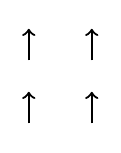
\begin{tikzpicture}
		\draw[thick,->] (0,0) -- (0,0.4);
		\draw[thick,->] (0,0.8) -- (0,1.2);
		\draw[thick,->] (0.8,0) -- (0.8,0.4);
		\draw[thick,->] (0.8,0.8) -- (0.8,1.2);
	\end{tikzpicture}
	,
	\hspace{1 cm}
	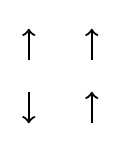
\begin{tikzpicture}
		\draw[thick,->] (0,0.4) -- (0,0);
		\draw[thick,->] (0,0.8) -- (0,1.2);
		\draw[thick,->] (0.8,0) -- (0.8,0.4);
		\draw[thick,->] (0.8,0.8) -- (0.8,1.2);
	\end{tikzpicture}
	,
	\hspace{1 cm}
	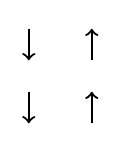
\begin{tikzpicture}
		\draw[thick,->] (0,0.4) -- (0,0);
		\draw[thick,->] (0,1.2) -- (0,0.8);
		\draw[thick,->] (0.8,0) -- (0.8,0.4);
		\draw[thick,->] (0.8,0.8) -- (0.8,1.2);
	\end{tikzpicture}
	,
	\hspace{1 cm}
	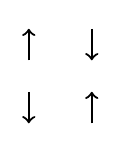
\begin{tikzpicture}
		\draw[thick,->] (0,0.4) -- (0,0);
		\draw[thick,->] (0,0.8) -- (0,1.2);
		\draw[thick,->] (0.8,0) -- (0.8,0.4);
		\draw[thick,->] (0.8,1.2) -- (0.8,0.8);
	\end{tikzpicture}
	,
	\hspace{1 cm}
	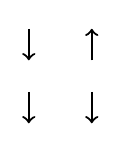
\begin{tikzpicture}
		\draw[thick,->] (0,0.4) -- (0,0);
		\draw[thick,->] (0,1.2) -- (0,0.8);
		\draw[thick,->] (0.8,0.4) -- (0.8,0);
		\draw[thick,->] (0.8,0.8) -- (0.8,1.2);
	\end{tikzpicture}
	,
	\hspace{1 cm}
	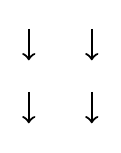
\begin{tikzpicture}
		\draw[thick,->] (0,0.4) -- (0,0);
		\draw[thick,->] (0,1.2) -- (0,0.8);
		\draw[thick,->] (0.8,0.4) -- (0.8,0);
		\draw[thick,->] (0.8,1.2) -- (0.8,0.8);
	\end{tikzpicture}
	,
\end{center}
\begin{center}
(a)
\hspace{1.6 cm}
(b)
\hspace{1.6 cm}
(c)
\hspace{1.6 cm}
(d)
\hspace{1.6 cm}
(e)
\hspace{1.6 cm}
(f)
\end{center}

where we have ordered the states from all spins up through all spins down. Note that there are two unique orientations with two spins up and two spins down. They are unique in terms of energy considerations, as shown in the table below. Another important property to consider is the magnetization of the system, determined as
\begin{equation}
M = \sum\limits^N_{i=1} s_i,
\end{equation}
where $s_i$ is the spin of the $i$th particle, as before. With this in mind, we construct a summary of the properties in Figure (1).
\begin{figure}
\centering
\begin{tabular}{| l | l | l | l | l |}
\hline
 & Spins Up & Count & Magnetization & Energy  \\ \hline
(a) & 4 & 1 & 4 & -8J \\ \hline
(b) & 3 & 4 & 2 & 0 \\ \hline
(c) & 2 & 4 & 0 & 0 \\ \hline
(d) & 2 & 2 & 0 & 8J \\ \hline
(e) & 1 & 4 & -2 & 0 \\ \hline
(f) & 0 & 1 & -4 & -8J \\ \hline
\end{tabular}
\caption{Here we compile the various important properties of the two-by-two spin system, letters referring to the diagram. Particularly important to distinguish are cases (c) and (d). Due to their configurations, they are unique in terms of count and energy configuration. Observe that in (c) each particle has two aligned and two anti-aligned neighbors with periodic boundary conditions, so the total energy is zero. In the case of (d), each particle's neighbors are all anti-aligned so we see the energy total is $8J$, the highest for the entire system.}
\end{figure}

For the Ising model we apply the Boltzmann distribution, wherein the probability of a given state is determined by its energy as
\begin{equation}
P(E_i) = \frac{e^{-E_i/T}}{\sum\limits^N_{i=1} e^{-E_i/T}} = \frac{e^{-E_i\beta}}{Z},
\end{equation}
where we define $\beta$ for convenience and $Z$ as a normalization factor,
\begin{equation}
\beta = \frac{1}{T}, \hspace{0.5 cm} Z = \sum\limits^N_{i=1} e^{-\beta E_i}.
\end{equation}
With this distribution and the information in Figure (1), we are able to determine the mean energy and magnetization of the system. Summing over all states, the mean energy is 
\begin{align*}
<E> &= \frac{1}{Z}\sum\limits^N=16_{i=1} E_i e^{-E_i\beta} \\
	&= \frac{1}{Z}\bigg( -8Je^{8J\beta} + 2(8J)e^{-8J\beta} + -8Je^{8J\beta} \bigg) \\
	&= \frac{-16J}{Z}\bigg(e^{8J\beta} - e^{-8J\beta}\bigg) \\
	&= \frac{-32J}{Z}sinh(8J\beta)
\end{align*}
and the mean magnetization is
\begin{align*}
<M> &= \frac{1}{Z}\sum\limits^{N=16}_{i=1} M_i e^{-E_i\beta} \\
	&= \frac{1}{Z}\bigg( 4e^{8J\beta} + 2(4) - 2(4) - 4e^{8J\beta} \bigg) \\
	&= 0.
\end{align*}
Noting that not only is the mean magentization zero but that any non-zero calculated will vary between negative and positive values of the same magnitude depending upon whether the system aligns up or down, each equal in energy and therefore probability, we instead calculate the mean absolute value of magnetization, as
\begin{align*}
<|M|> 	&= \frac{1}{Z}\bigg( 4e^{8J\beta} + 4(2) + 4(2) + 4e^{8J\beta} \bigg) \\
		&= \frac{-16J}{Z}\bigg(8e^{8J\beta} + 16\bigg) \\
		&= \frac{8}{Z}\bigg(e^{8J\beta} + 2\bigg).
\end{align*}
Deriving the partition function as 
\begin{equation}
Z = e^{-8J\beta} + 4 + 4 + 2e^{8J\beta} + 4 + e^{-8J\beta} = 12 + 3cosh(8J\beta)
\end{equation},
we arrive at our final expressions for the mean energy and mean absolute magentization as
\begin{equation}
<E> = -8J\frac{sinh(8J\beta)}{3 + cosh(8J\beta)}
\end{equation}
and
\begin{equation}
<|M|> = \frac{2e^{8J\beta} + 4}{3+cosh(8J\beta)},
\end{equation}
respectively.

With these calculated, we turn our attention to the heat capacity, $C_v$, and magnetic susceptibility, $\chi$, defined as
\begin{equation}
C_v = \frac{1}{T^2}\bigg(<E^2> - <E>^2\bigg)
\end{equation}
and
\begin{equation}
\chi = \frac{1}{T}\bigg(<M^2> - <|M|>^2\bigg),
\end{equation}
where we have used $<|M|>$ in place of the normal $<M>$ for the magnetic suspceptibility for the reasons stated above. Deriving 
\begin{equation}
<E^2> = 64J^2\frac{cosh(8J\beta)}{3+cosh(8J\beta)}
\end{equation}
and
\begin{equation}
<M^2> = \frac{8e^{8J\beta} + 8}{3 + cosh(8J\beta)},
\end{equation}
we find that
\begin{equation}
C_v = 64J^2\frac{3cosh(8J\beta) + 1}{(3 + cosh(8J\beta))^2}
\end{equation}
and
\begin{equation}
\chi = 4\frac{2sinh(8J\beta) + 4cosh(8J\beta) + 3)}{(3 + cosh(8J\beta))^2}.
\end{equation}

From here, we divide by the total number of spins as a mean of comparing systems of differing sizes, resulting in our final forms of
\begin{equation}
\frac{<E>}{N} = -2J\frac{sinh(8J\beta)}{3 + cosh(8J\beta)},
\end{equation}

\begin{equation}
\frac{<|M|>}{N} = \frac{1}{2}\frac{e^{8J\beta} + 2}{3+cosh(8J\beta)},
\end{equation}

\begin{equation}
\frac{C_v}{N} = 16J^2\frac{3cosh(8J\beta) + 1}{(3 + cosh(8J\beta))^2},
\end{equation}

\begin{equation}
\frac{\chi}{N} = \frac{2sinh(8J\beta) + 4cosh(8J\beta) + 3}{(3 + cosh(8J\beta))^2}.
\end{equation}

These results will be used as the exact answer for comparison with the algorithm and code discussed in the next section.

\section{Methodology}

In this section we discuss and implement an agorithm to calculate the desired quantities for the 2D Ising Model. My own code written for this task is included in my github repository, as seen at the beginning of the project, which includes options for outputting files for the probability distribution of energies, computing each mean quantity as a function of monte carlo cycles, and as each mean quantity as a function of temperature.

\subsection{Metropolis Algorithm and Detailed Balance}

In principle calculating the partition function, or weighting function, is straightforward, but in practice it quickly becomes unmanageable. For the two-by-two case there exist only $2^4$ cases to sort through, but as we increase the grid size the number of possible configurations grows exponentially, as $2^{(n^2)}$, so as we reach a twenty-by-twenty grid, we have $2^{400}$ possible configurations, or ~$2.5*10^{120}$. This is far too many configurations to sort through and so we turn to the Metropolis Algorithm and Detailed Balance in order to avoid the need of calculating the partition function.

In order to apply the Metropolis Algorithm we required that two conditions be fulfilled, first that there exist some stationary distribution $\pi$(x) which fulfills the condition of detailed balance, that is that the transition from each state $x$ to each other state $x'$ is reversible,
\begin{equation}
\pi(x)P(x \rightarrow x') = \pi(x')P(x'\rightarrow x),
\end{equation}
where P(x $\rightarrow$ x') is the probability of transitioning from a state $x$ to a state $x'$. This is a necessary but not sufficient condition. Secondly we require that the stationary distribution is unique. This condition is met by requiring the system be ergodic, that is that the system must be aperiodic, not return to the same state at fixed intervals, and that it is positive recurrent, that the number of steps for returning to the same state is finite. A simple way to consider this condition is that any one state must be reachable by any another state by a finite number of steps; there can be no closed loops or fixed paths. With these two conditions fulfilled we can begin from the statement of detailed balance to calculate the transition probabilities from one state to another.

Beginning from the statement of detailed balance, choosing to represent the unknown distribution $\pi$(x) with $P$(x), we rewrite the equation to obtain
\begin{equation}
\frac{P(x)}{P(x')} = \frac{P(x' \rightarrow x)}{P(x \rightarrow x')}.
\end{equation}
Next, since we do not know the transition probabilities, we choose to model them in terms of a multiplication of two quantities, the proposal distribution, $g$, and the acceptance distribution, $A$, as
\begin{equation}
P(x \rightarrow x') = g(x \rightarrow x')A(x \rightarrow x'),
\end{equation}
so that
\begin{equation}
\frac{P(x)}{P(x')} = \frac{g(x' \rightarrow x)A(x' \rightarrow x)}{g(x \rightarrow x')A(x \rightarrow x')}.
\end{equation}
The simplest method for choosing $g$ is to apply a normal distribution, that is we say the probability of selecting any one state is equal, or one over the total number of states, so that $g(x \rightarrow x')$ = $g(x' \rightarrow x)$, whence
\begin{equation}
\frac{P(x)}{P(x')} = \frac{A(x' \rightarrow x)}{A(x \rightarrow x')}.
\end{equation}
We know the stationary distribution to be given by the Boltzmann distribution, that is 
\begin{equation}
\frac{A(x' \rightarrow x)}{A(x \rightarrow x')} = \frac{P(x)}{P(x')} = \frac{e^{-E_x\beta}/Z}{e^{-E_{x'}}/Z} = e^{-\big(E_x - E_{x'}\big)\beta} = e^{-\Delta E_{xx'}\beta}.
\end{equation}
We assume that the system will naturally gravitate towards lower energies, so we state without loss of generality that $E_{x'} \leq E_x$, resulting in $\Delta E_{xx'} \geq$ 0. Since we now have a ratio between the acceptance probabilities from $x \rightarrow x'$ and $x' \rightarrow x$, we set the acceptance probability which reduces or maintains energy to one, here $A(x \rightarrow x')$ = 1. Then
\begin{equation}
A(x \rightarrow x') = 1
\end{equation}
and
\begin{equation}
A(x' \rightarrow x) = e^{-\Delta E_{xx'}\beta},
\end{equation}
so that we have defined the transition probability between any two states. 

\subsection{Monte Carlo method}

With our selection distribution, $g$, and our acceptance distribution, $A$, chosen we are able to implement the Monte Carlo method for evolving the system. 

It is simple in theory; we select a spin, $s_i$, according to our distribution $g$, here defined to be normal so each spin is weighted equally, and we test flipping it against our distribution $A$. If flipping the spin will lower or maintain the energy, we accept it. If it will raise the energy, we accept it will probability $e^{-\Delta E\beta}$. If the change is accepted, we flip the spin and update the energy and magnetization accordingly. If it is denied, the system remains as it was. We define a number of such selections and tests equal to the number of spins to be one full Monte Carlo cycle.

Outling the basic methodology, we
\begin{enumerate}
\item[1.]
Select a random spin $s_i$.
\item[2.]
Calculate $\Delta E$
\item[3.]
If $\Delta E \leq$ 0, accept the change. Update the system.
\item[4.]
If $\Delta E >$ 0, accept the change with probability $e^{-\Delta E\beta}$. Update the system accordingly.
\item[5.]
Repeat steps 1-4 $n^2$ times per MC cycle for a square n-by-n grid.
\item[6.]
Repeat steps 1-5 until the system reaches equilibrium.
\end{enumerate}

\subsection{Coding}

Here we discuss how to code the Metropolis algorithm outlined above.

We first generate a matrix of spin values, represented as +1 for spin up and -1 for spin down. We then proceed through the list provided above with slight alterations to clarify the tests involved. Note that the mean energy, mean magentization, and other mean values must only be updated after one full monte carlo cycle. This provides a much more stable and representative picture of the system. Updating after each individual test allows for far too high a variation, whereas updating after one full cycle helps to average out random fluctuations.

\begin{enumerate}
\item[1.]
Generator random numbers x, y $\in$ [0,n-1] according to a normal distribution. Select spin $s_{xy}$.
\item[2.]
Calculate $\Delta E$.
\item[3.]
If $\Delta E \leq$ 0, accept the change. Update the energy and magnetization of the system.
\item[4.]
If $\Delta E >$ 0, generator a random number z $\in$ [0.0,1.0] according to a normal distribution. Accept the change if z $\leq e^{-\Delta E\beta}$. Update the system accordingly.
\item[5.]
Repeat steps 1-4 $n^2$ times per MC cycle for a square n-by-n grid.
\item[6.]
Update the desires mean values.
\item[7.]
Repeat steps 1-6 for the desired number of MC cycles.
\item[8.]
Divide the mean values by the number of MC cycles.
\item[9.]
Calculate heat capacity and magnetic susceptibility from the necessary mean values.
\end{enumerate}

\section{Results}

Here we begin by testing the algorithm against the exact two-by-two solutions from the previous in the paper and follow it with tests of computational speed. We then proceed to testing various grid sizes in search of the critical temperature in the infinite limit. The code for these results can be found at my github address as included in the beginning of this paper. In project4.cpp options are included for output of probability distributions, a loop through numbers of monte carlo cycles, and a loop through temperature values. Instructions are included therein.

In Figure (1) we compare the mean energy, mean magnetization, heat capacity, and magnetic susceptibility for the two-by-two case with the exact solutions. In Figure (2) we test the scaling of the algorithm by varying both grid size and the number of monte carlo cycles. In Figures (3) and (4) we see effects of beginning with aligned or unaligned for various temperatures. In Figure (5) we observe the effect on the number of accepted states as a function of monte carlo cycles by varying temperature. In Figures (6) and (7) we plot the probability distributions of the 20-by-20 grid for varying temperatures. In Figures (8) through (11) we see the mean energy, mean magnetization, heat capacity, and magnetic susceptibility as functions of temperature for varying grid sizes. In Figures (12) and (13) we plot the heat capacity and magnetic susceptibility from (10) and (11) with a finer step size in search of the critical temperature for each grid size. In Figure (14) we compile the critical temperatures from the plots of (12) and (13). In Figure (15) we plot the data from (14) and fit linear regressions to retrieve the critical temperature in the infinite limit.
 
\begin{figure}
\center
\begin{tabular}{| l | l | l | l | l | l |}
\hline
          
$2^i$     &       cycles      &          $E$/N      &    $|M|$/N   &    $C_v$/N      &     $\chi$/N	\\ \hline
7       &     128     &  	  -1.96875  &    0.992188   &   0.246094  &    0.0153809 \\ \hline
8       &     256     &     -1.96875  &   0.990234     & 0.246094    &  0.0269623 \\ \hline
 9      &      512     &      -1.98438   &   0.993164    & 0.124023    &  0.0252037\\ \hline
10     &      1024     &       -1.99609   &   0.999023    & 0.031189    & 0.00194931\\ \hline
11     &      2048     &  -1.99219   &   0.997803   &  0.0622559   &  0.00535178\\ \hline
 12     &      4096     &      -1.99707   &   0.999023   &  0.0234032   &  0.00292587\\ \hline
13    &       8192     &      -1.9978    &   0.99939    &  0.0175588   &  0.00146335\\ \hline
14    &      16384     &      -1.99438   &   0.998108   &  0.0447958   &  0.00572298\\ \hline
15    &      32768     &      -1.99518   &   0.998444   &  0.0384812   &  0.00450691\\ \hline
16   &       65536     &      -1.99655     &   0.998833   &   0.0275403  &   0.00354985\\ \hline
 17   &      131072     &         -1.99582   &   0.998604   & 0.0333773    & 0.00418837\\ \hline
 18   &      262144     &       -1.99589   &     0.998604 &    0.0328303 &    0.00425703\\ \hline
19   &      524288     &      -1.99582   &    0.998618  &     0.033347 &    0.00410651\\ \hline
20   &     1048576     &      -1.99582     & 0.998609    & 0.0333622     &0.00416172\\ \hline
\end{tabular}
\caption{A table summarizing the desired values after a given number of monte carlo cycles. Column one indicates the power to which two was raised to obtain the listed number of cycles. The exact answers from section two for T=1.0, J=1.0 are E = -1.996, M = 0.999, $C_v$ = 0.0322, and $\chi$ = 0.00401. Note that since we've set T=1.0 and J=1.0 that $C_v$ and $\chi$ double numerically as the varience of E and M, respectively. From this table it seems clear we require at least $2^{18}-2^{20}$ monte carlo cycles before we may be confident in the results.}
\end{figure}
\begin{figure}
\centering
\begin{tabular}{| l | l | l | l | l | l | l |}
\hline
$2^i$     &       cycles   & 	time(2)[s]		&time(20)[s]	&time(40)[s]&	time(60)[s]&time(80)[s] 	\\ \hline	
10    &       1024   &   0.001475  &  0.136543   & 0.552883	&1.22494 	&	2.21758 \\ \hline
11    &       2048   &   0.002992  &  0.27044    &	1.1052 	&	2.4495 		&	4.45527 \\ \hline
12    &       4096   &   0.005969  &  0.551546   &	2.19842	&	4.99269 	&	8.92798 \\ \hline
13    &       8192   &   0.012101  & 	1.12443   &  4.40526 &	9.96672		&	17.7866\\ \hline
14    &      16384   &   0.024321  &  2.1936 	&	8.86753 &	19.7791 	&	35.4322 \\ \hline
15    &      32768   &   0.048069  &  4.36856	&	17.6465  &	39.5668 	&	71.1234 \\ \hline
\end{tabular}
\caption{A table summarizing the computation time of the program. The first column indicates the power to which two is raised to obtain the number of cycles. There is a clear linear trend between the number of operations and the computation time, displayed in two ways. First, observe for each column that as the number of cycles is doubled the computation time doubles as well. Second, as the grid size is increased a linear increase in time is observed. From 2 to 20 there is a hundredfold increase in the number of operations per cycle and the time is increased by approximately 100. From 20 to 40, there is a fourfold increase and a near quadrupling in the time. From 40 to 60 there is a 9/4 increase and from 60 to 80 a 16/9 increase both spin counts and computation times. So we see that a tenfold increase in grid size (side length) and cycle count would lead to a thousandfold increase in computation time, one hundred from an increase in spins and ten from cycles.}
\end{figure}
\begin{figure}
\centering
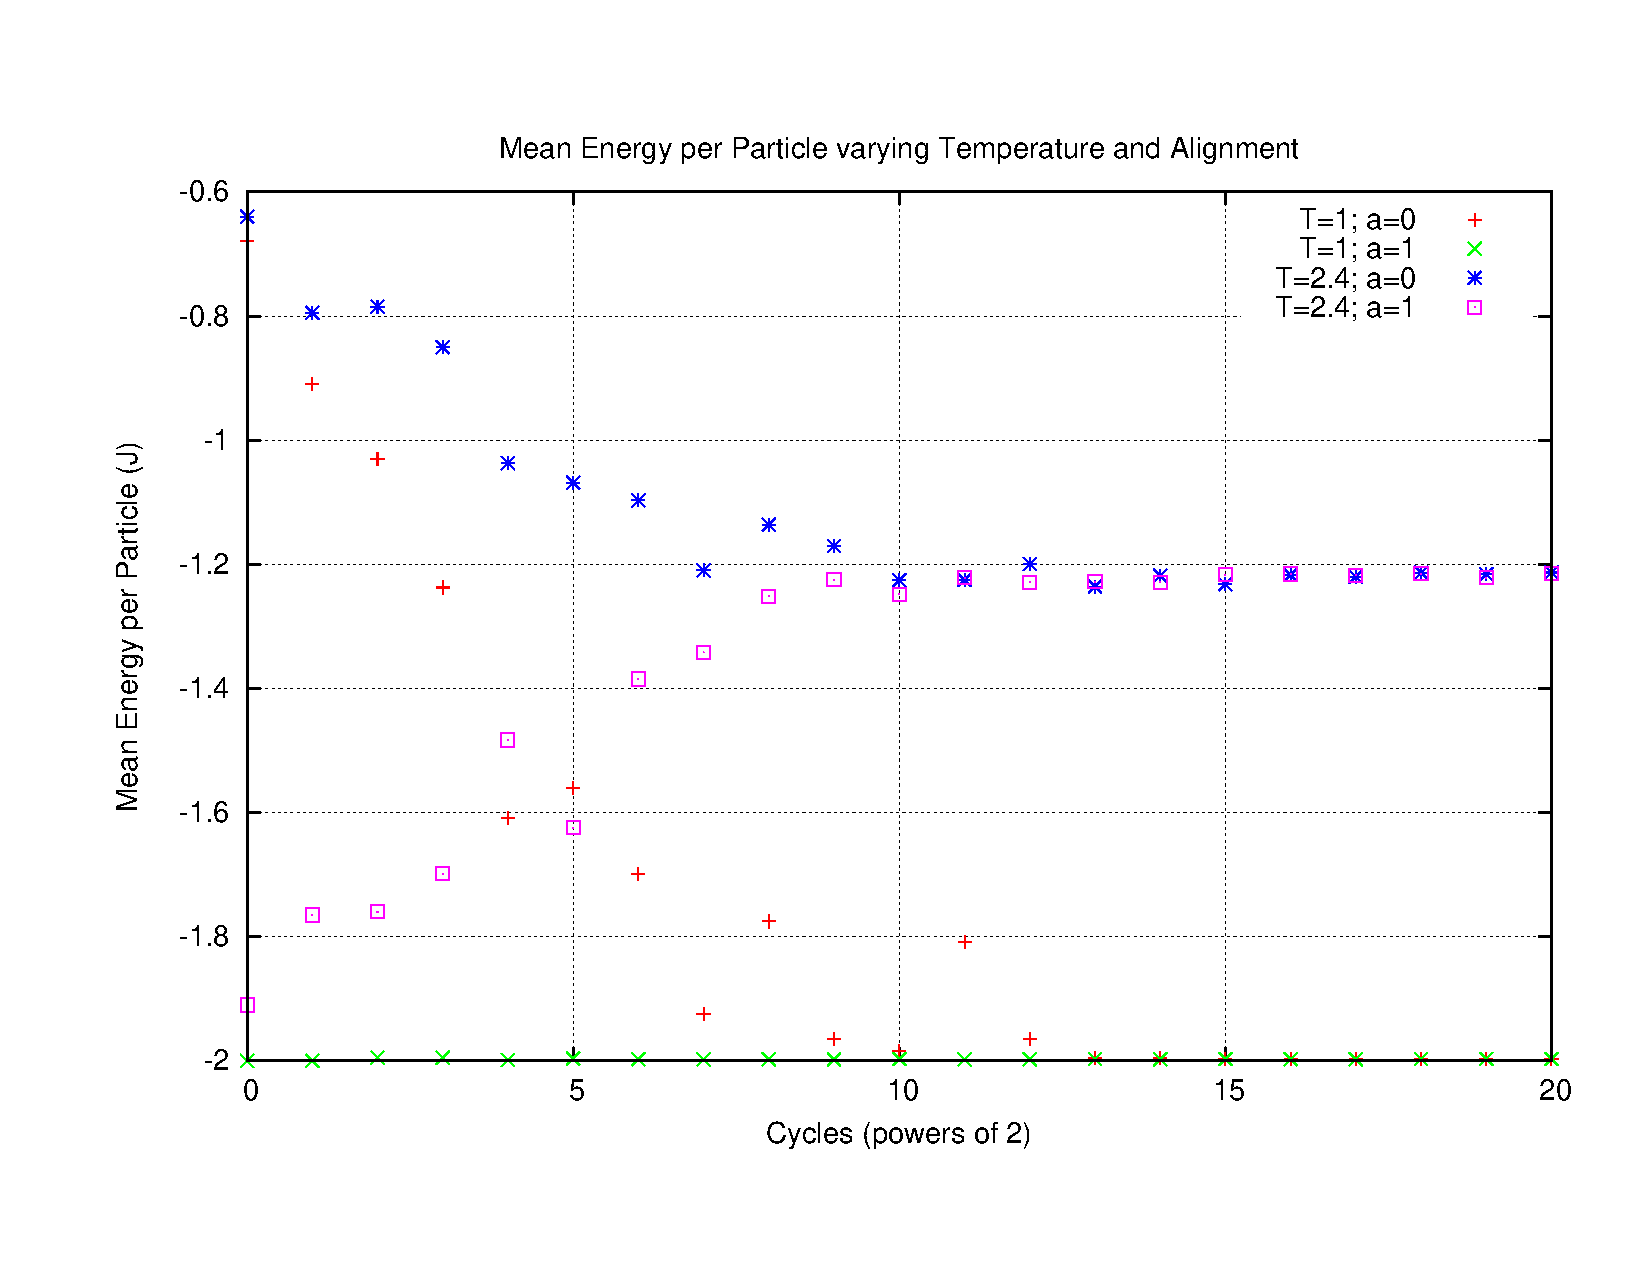
\includegraphics[width=1.0\textwidth]{n20_meanenergy.pdf}
\caption{Here we see the mean energy of the 20x20 system plotted as a function of cycles, cycles = $2^x$, while varying the temperature and alignment. We see that there is a clear distinction between the speed of attaining equilibrium for each alignment (random or fully aligned) depending upon the temperature. For T=1.0 the system has near-perfect alignment as its equilibrium so starting the system there is reasonable as the faster method of calculating the mean quantities. For T=2.4, however, the system is only partially aligned so one method is approximately equal in times of the required cycles.}
\end{figure}
\begin{figure}
\centering
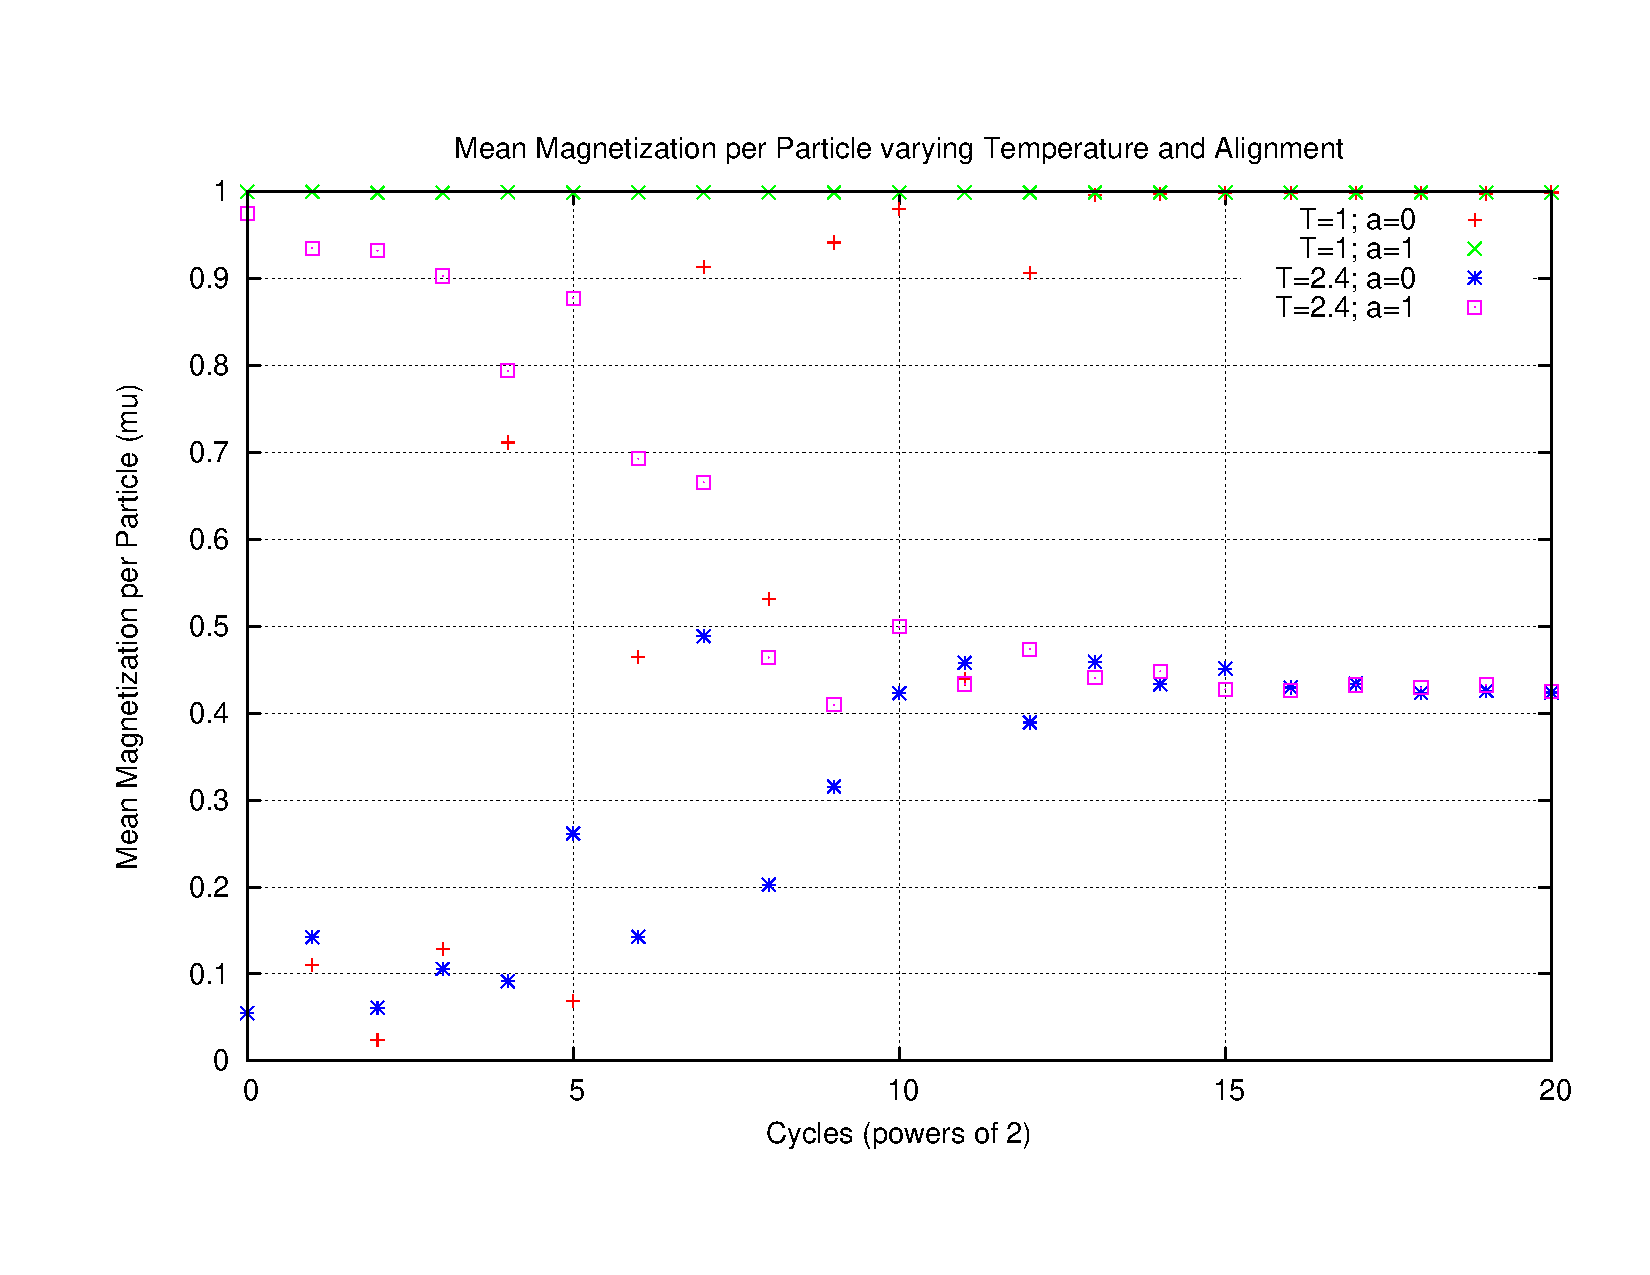
\includegraphics[width=1.0\textwidth]{n20_meanmag.pdf}
\caption{Here we see the mean magnetization of the 20x20 system plotted as a function of cycles, cycles = $2^x$, while varying the temperature and alignment. We see that there is a clear distinction between the speed of attaining equilibrium for each alignment (random or fully aligned) depending upon the temperature. For T=1.0 the system has near-perfect alignment as its equilibrium so starting the system there is reasonable as the faster method of calculating the mean quantities. For T=2.4, however, the system is only partially aligned so one method is approximately equal in times of the required cycles.}
\end{figure}
\begin{figure}
\centering
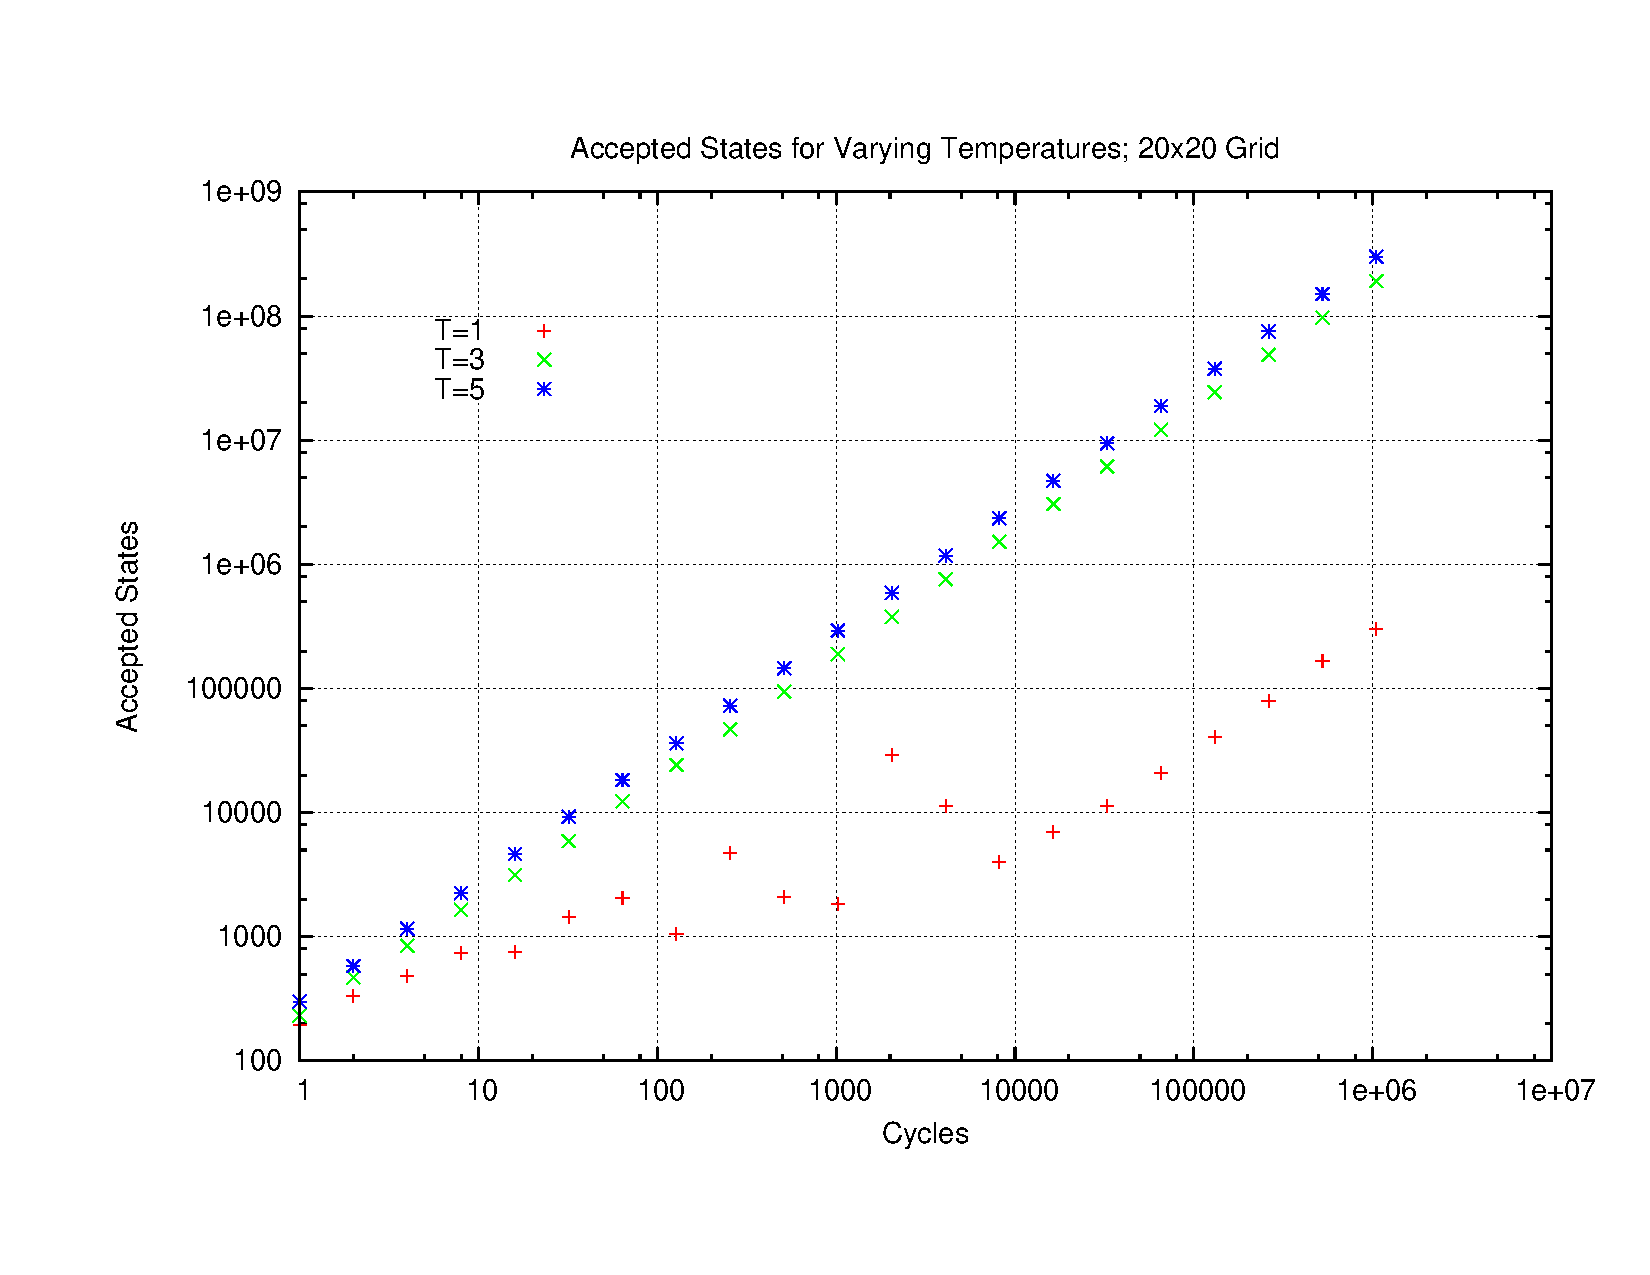
\includegraphics[width=1.0\textwidth]{accstates_loglog.pdf}
\caption{Here we see for a 20x20 grid the number of accepted states as a function of cycles while varying temperature. We see from the slope of the log-log plot that the relationship is clearly linear with the slope increasing as T increases, as indicated by the intercept of the graph. As T $\rightarrow \infty$, the slope of the linear curve should approach 400 as each state becomes more and more similar in terms of probability, making nearly every tested state accepted.}
\end{figure}
\begin{figure}
\centering
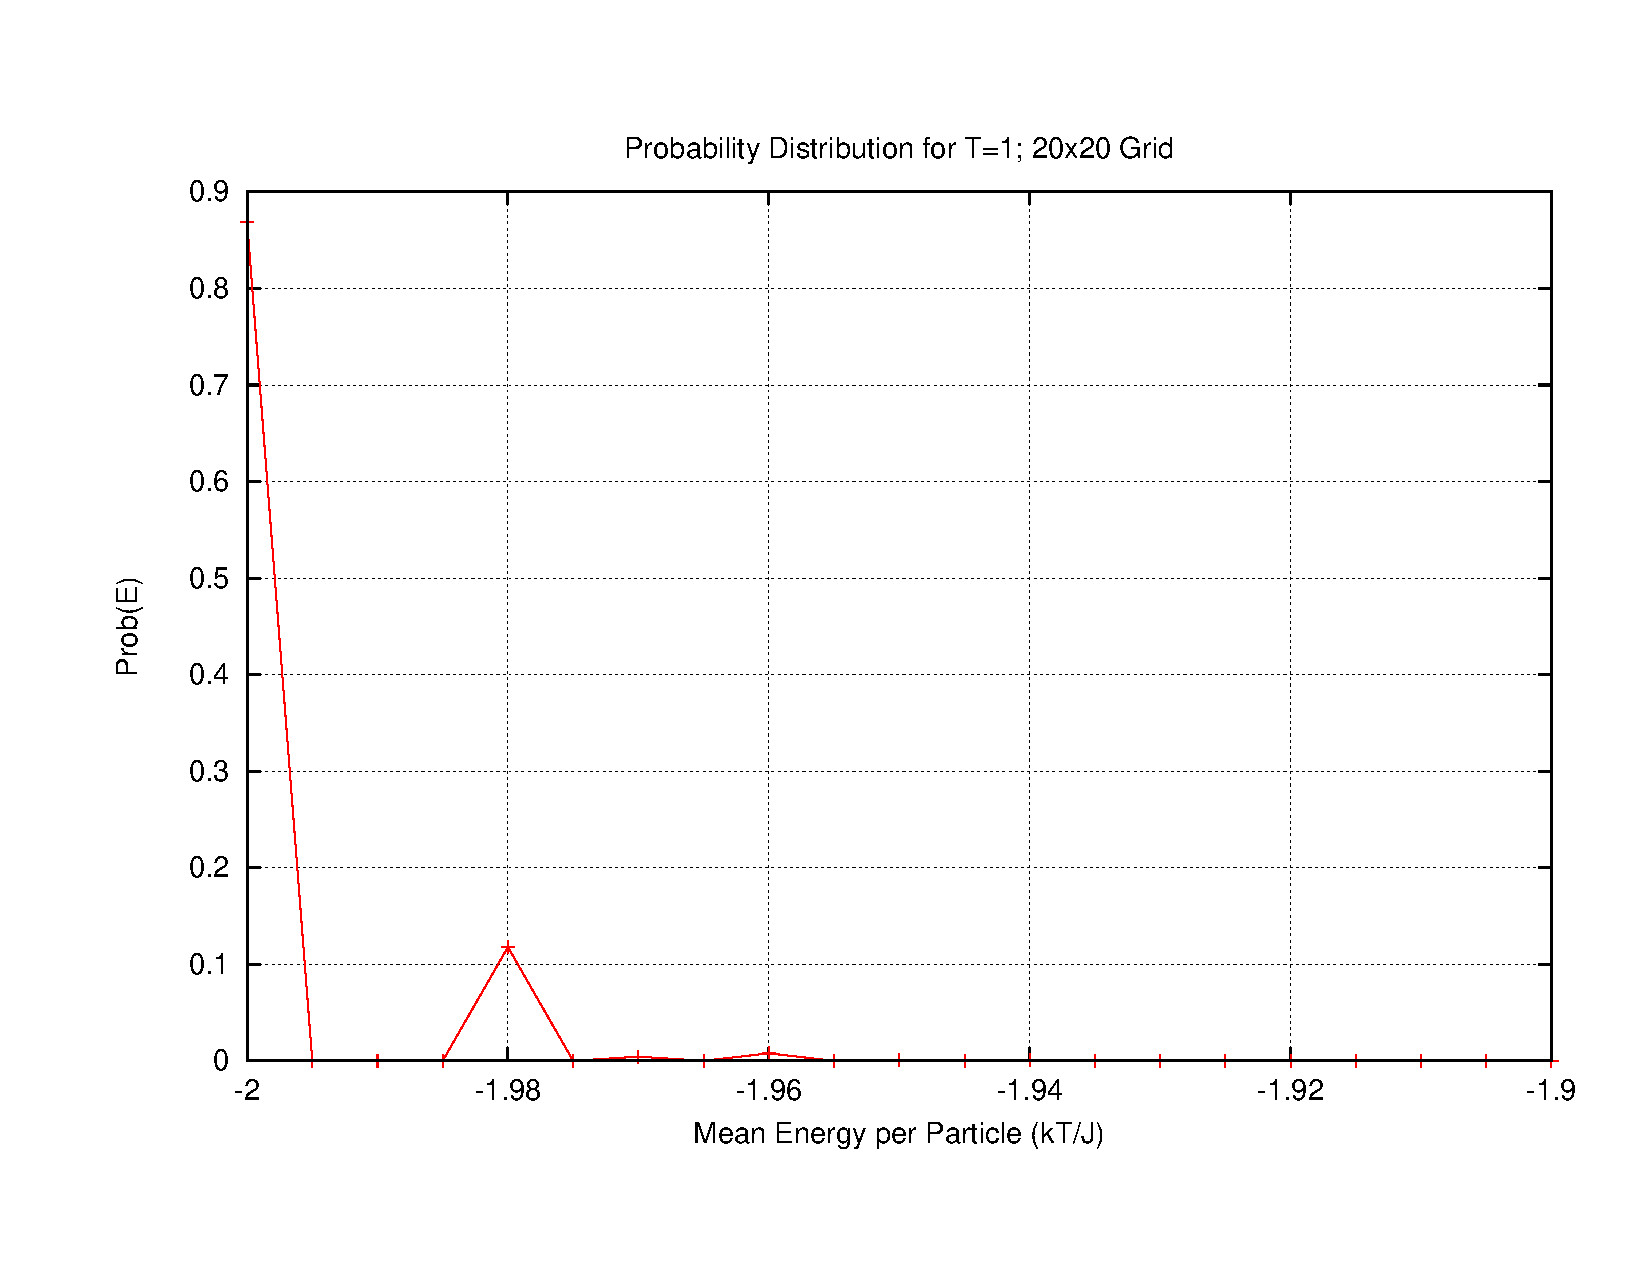
\includegraphics[width=1.0\textwidth]{prob_T1.pdf}
\caption{Here we see the probability distribution for a 20x20 grid with T=1. We see clearly that by far the most likely state is $E$/N = -2. The next most possible state is $E$/N = -1.98 reflecting that the only change from fully aligned to one misaligned involves a shift of eight energy units for the total system. The likelihood quickly decreasing as energy increases.}
\end{figure}
\begin{figure}
\centering
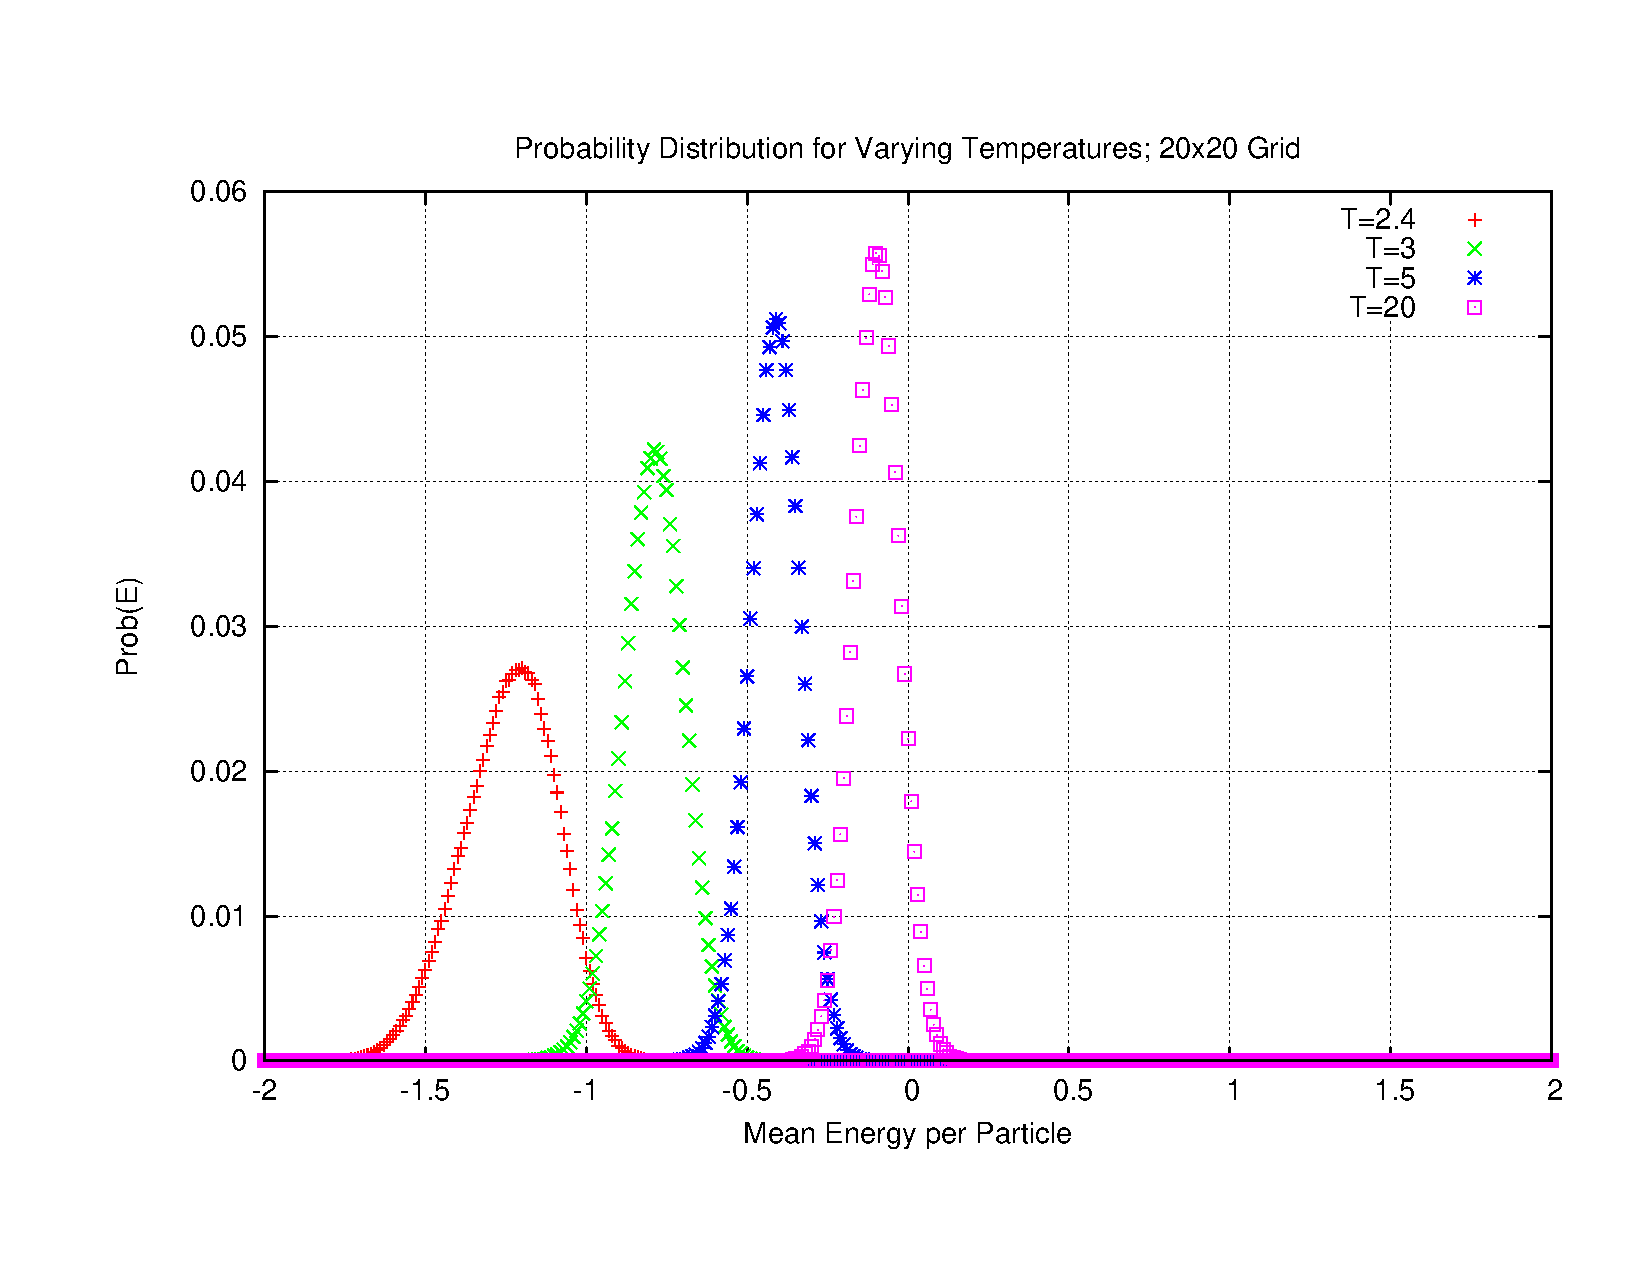
\includegraphics[width=1.0\textwidth]{prob_vT.pdf}
\caption{Here we see the probability distributions for a 20x20 grid with varying temperatures. Note that as T increases, the distribution shifts closer to having a mean value of zero and a thinner spread. This matches well the output data since we see a decrease in the variances of both $E$ and $M$ as T increases. This leads to a more focused distribution centered around zero, as we'd expect.}
\end{figure}
\begin{figure}
\centering
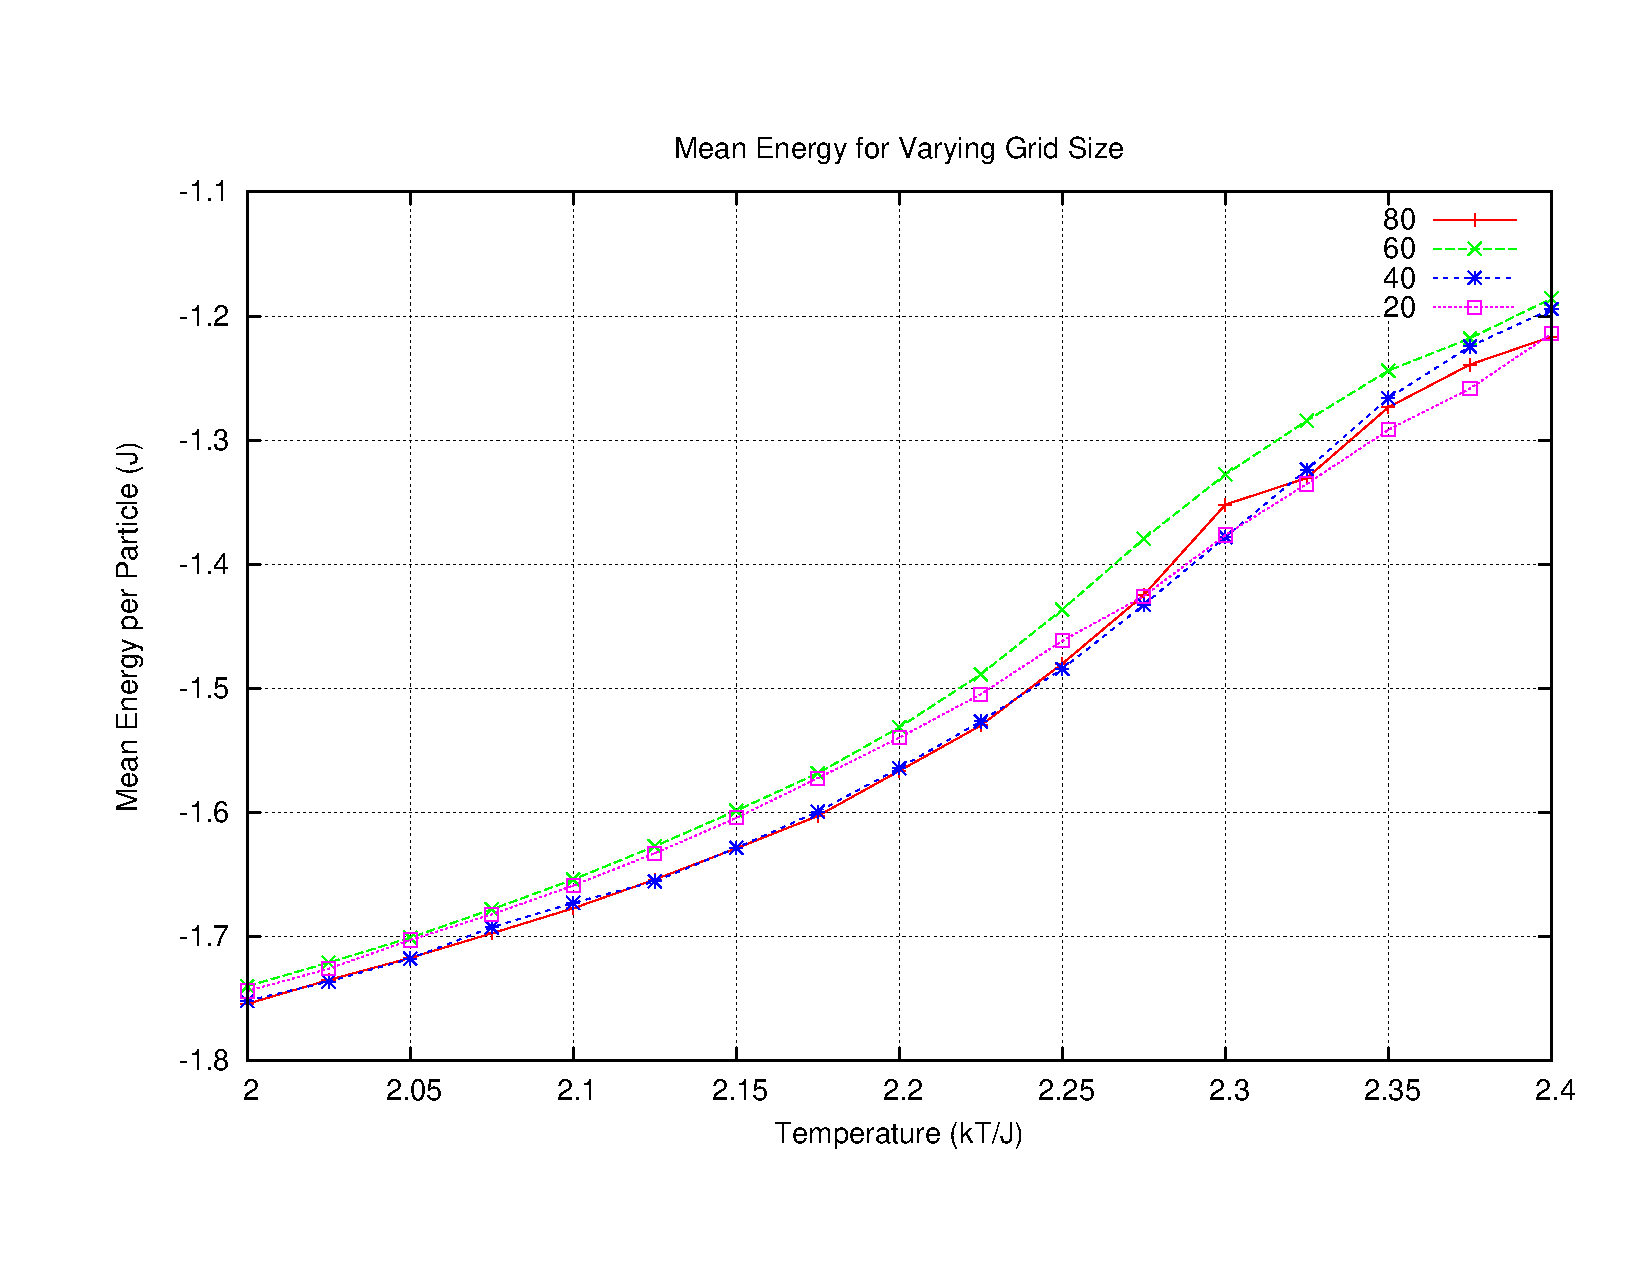
\includegraphics[width=1.0\textwidth]{meanenergy.pdf}
\caption{Here we see the mean energy over a range of temperatures with varying grid size. Note that near T=2.25 there is a change in the concavity of the mean energy curve. This is indicative of a phase transition.}
\end{figure}
\begin{figure}
\centering
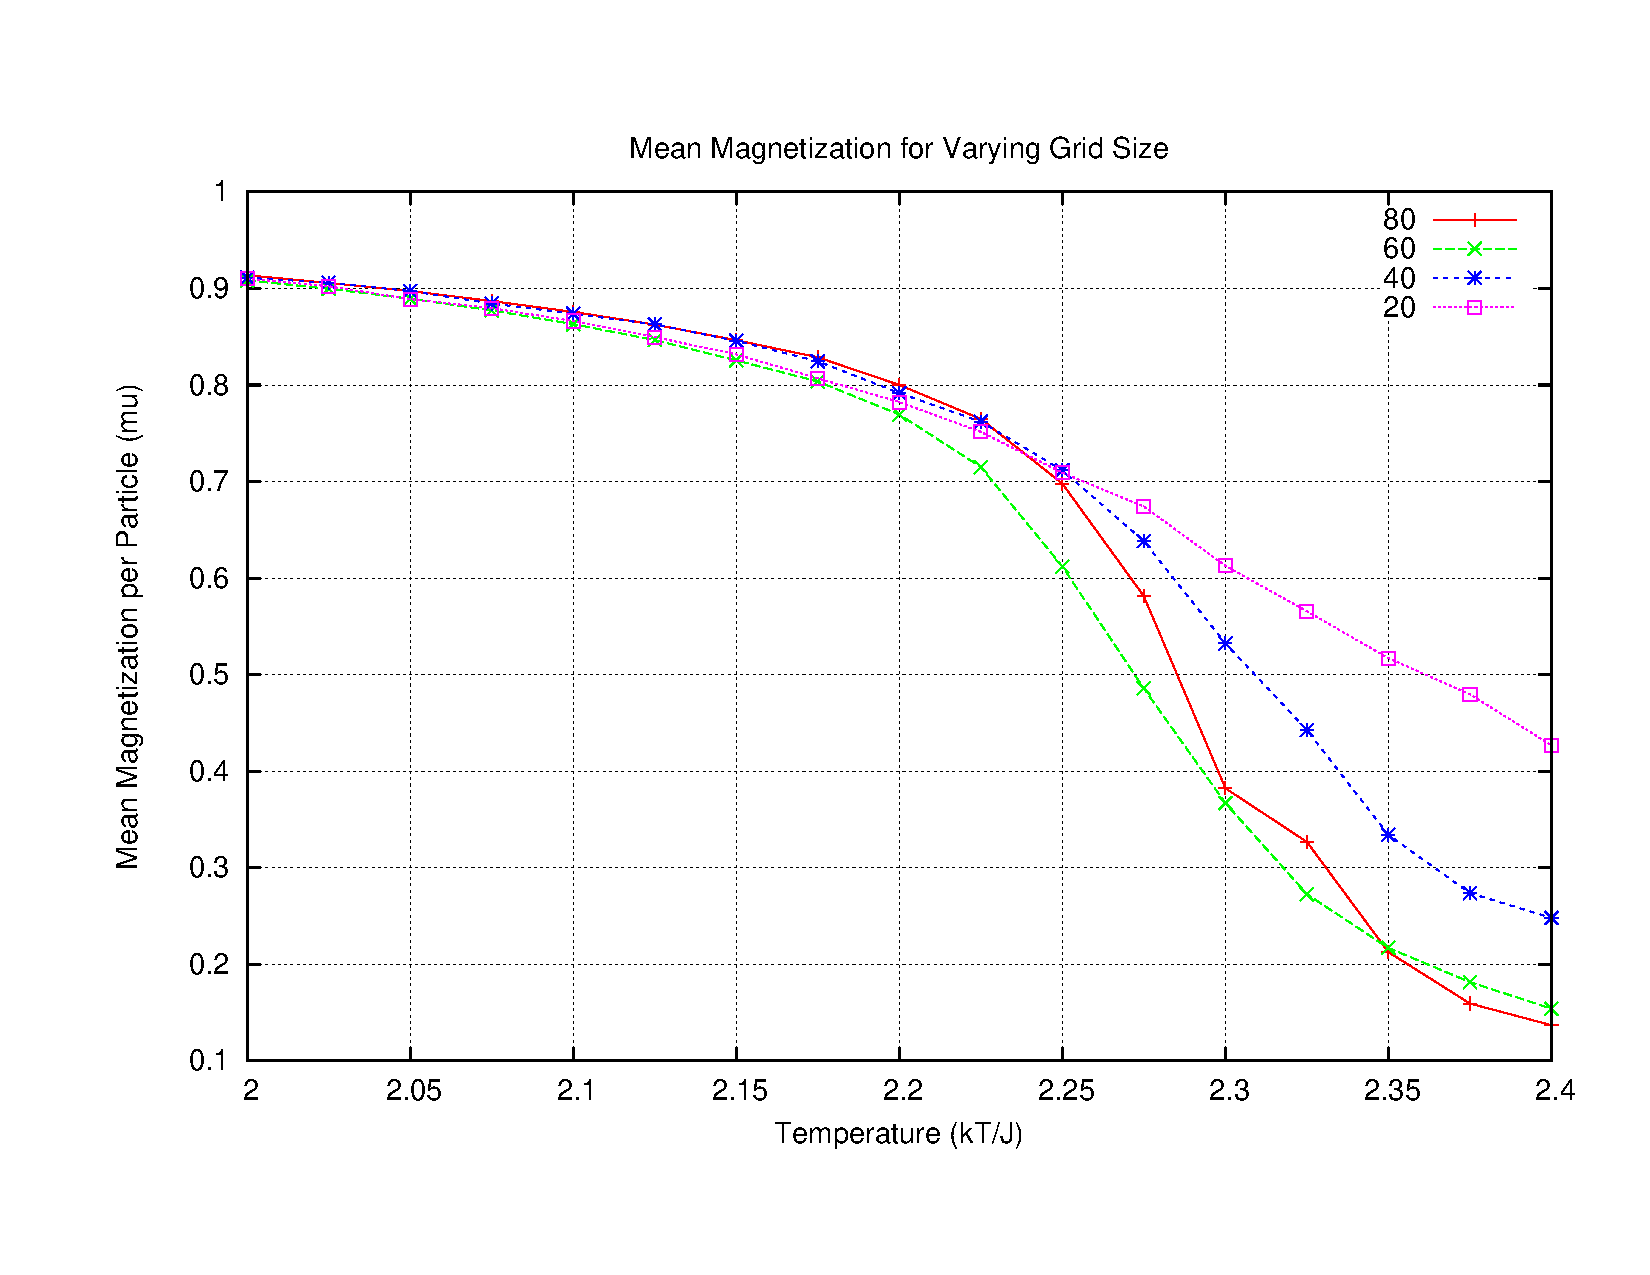
\includegraphics[width=1.0\textwidth]{meanmag.pdf}
\caption{Here we see the mean magnetization over a range of temperatures with varying grid size. Note that near T=2.3 there is a change in the concavity of the mean magnetization curve. This is indicative of a phase transition.}
\end{figure}
\begin{figure}
\centering
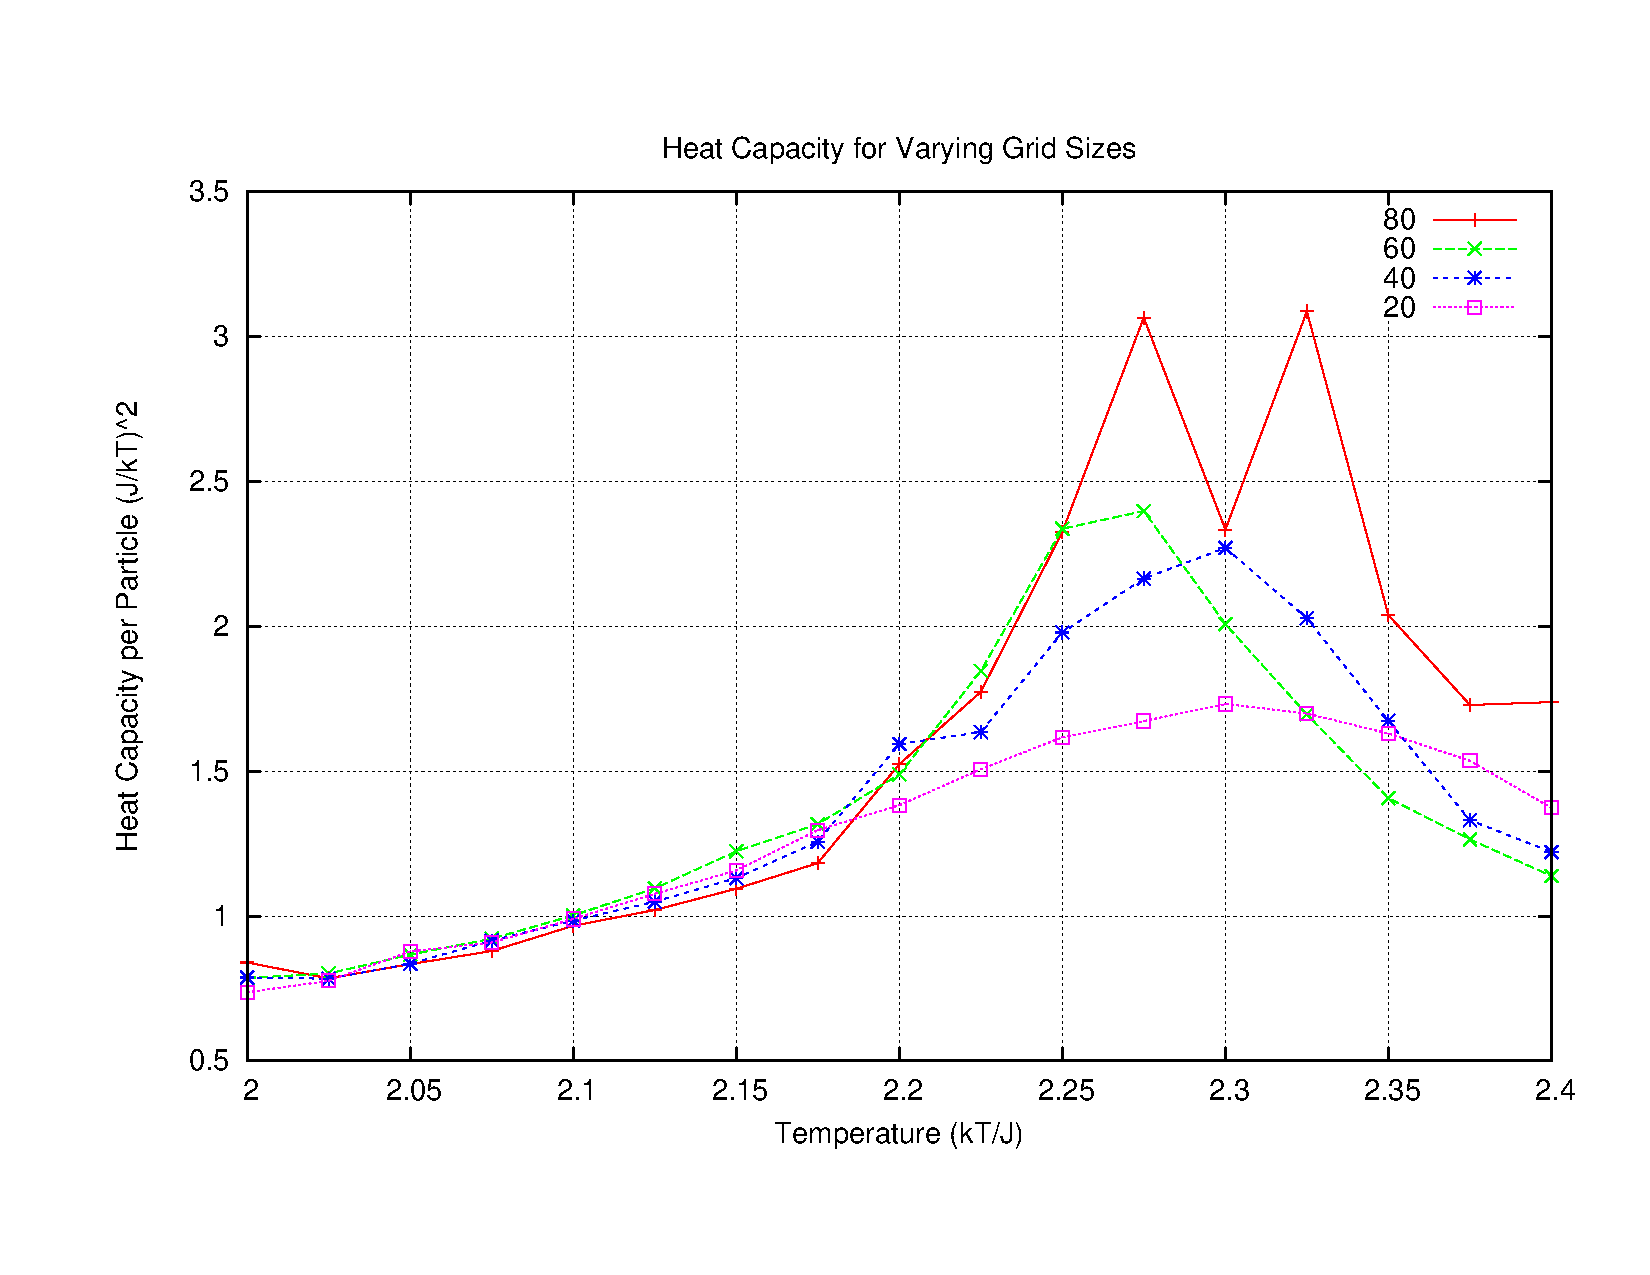
\includegraphics[width=1.0\textwidth]{heatcapacity.pdf}
\caption{Here we see the heat capacity as a function of temperature for varying grid sizes. We observe that the heat capacity has a peak which shifts leftward as temperature increases, again around T=2.25 - 2.3, again indicative of a phase transition. We will calculate with a finer step size the range between T=2.25 and T=2.35.}
\end{figure}
\begin{figure}
\centering
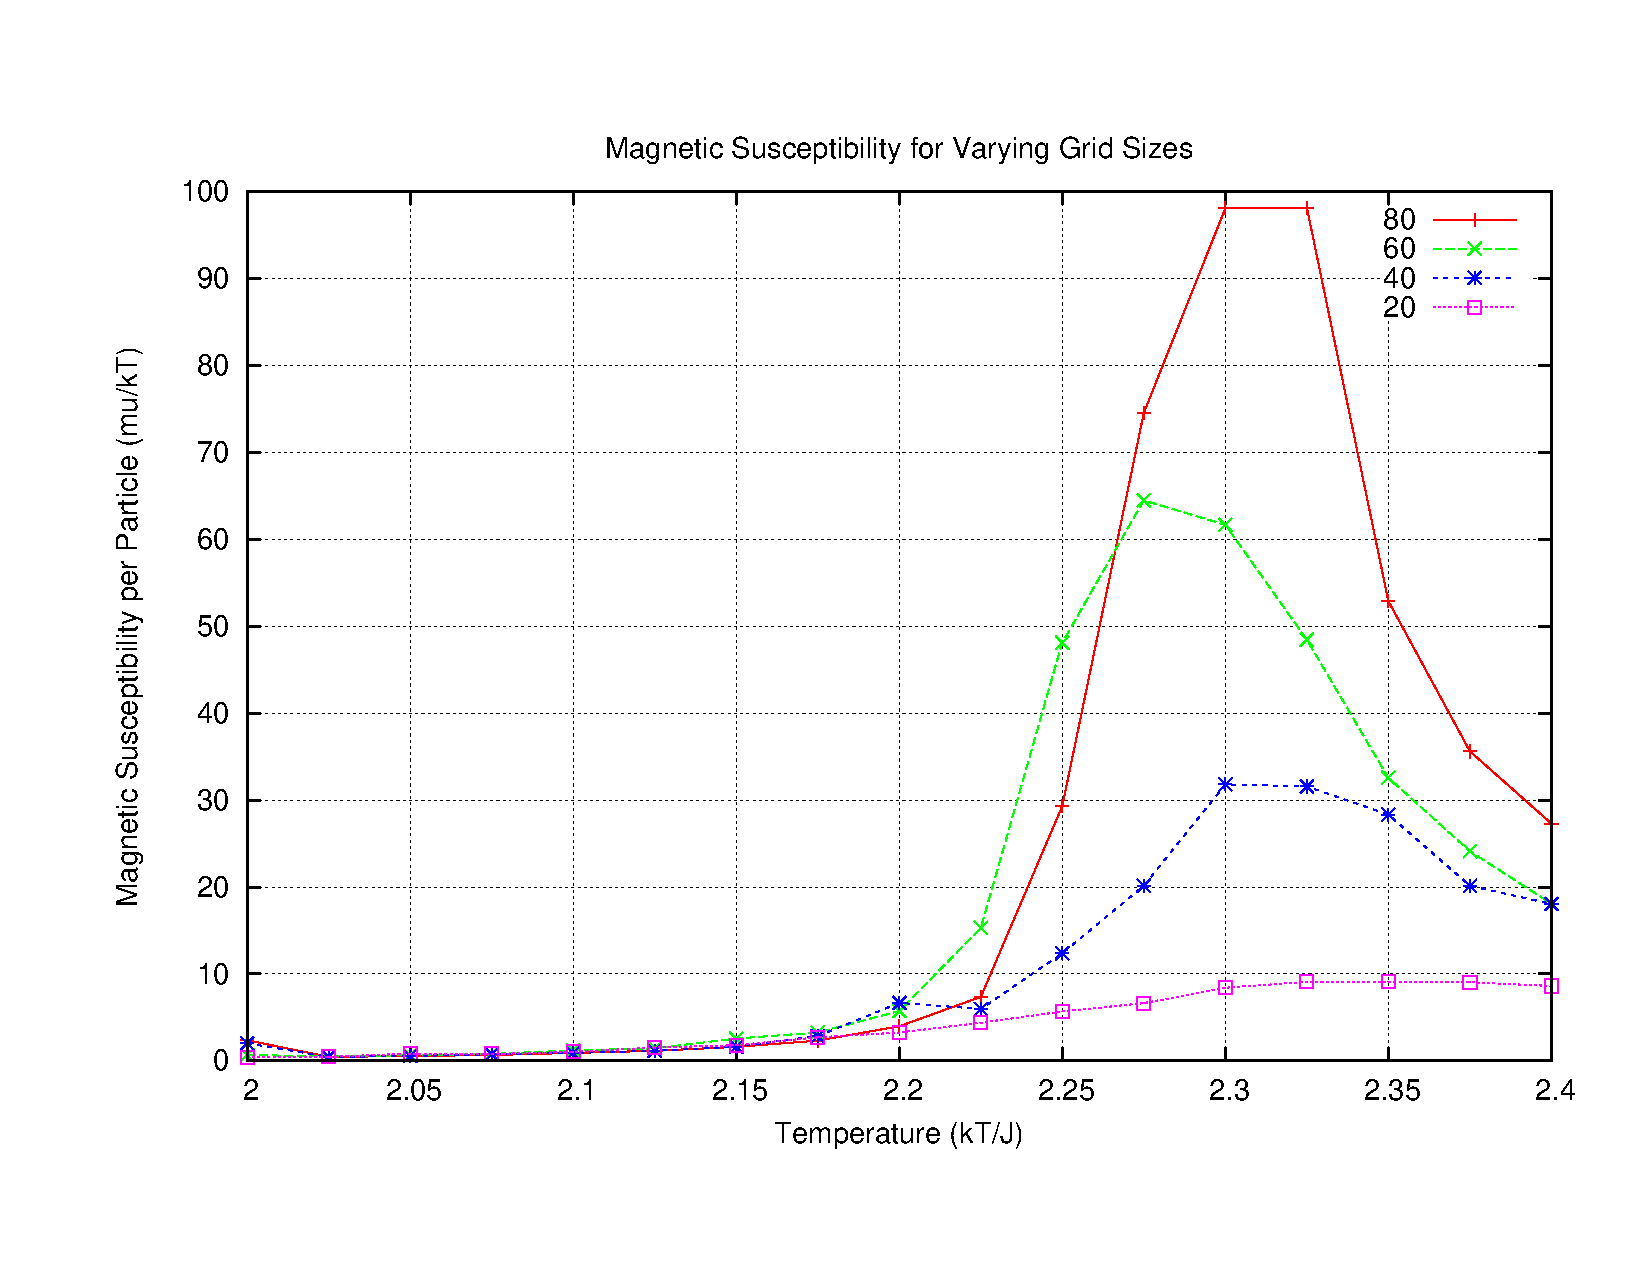
\includegraphics[width=1.0\textwidth]{magsus.pdf}
\caption{Here we see the magnetic susceptibility as a function of temperature for varying grid sizes. We observe that the magnetic susceptibility also has a peak which shifts leftward as temperature increases, again around T=2.25 - 2.3, again indicative of a phase transition. We will calculate with a finer step size the range between T=2.25 and T=2.35.}
\end{figure}
\begin{figure}
\centering
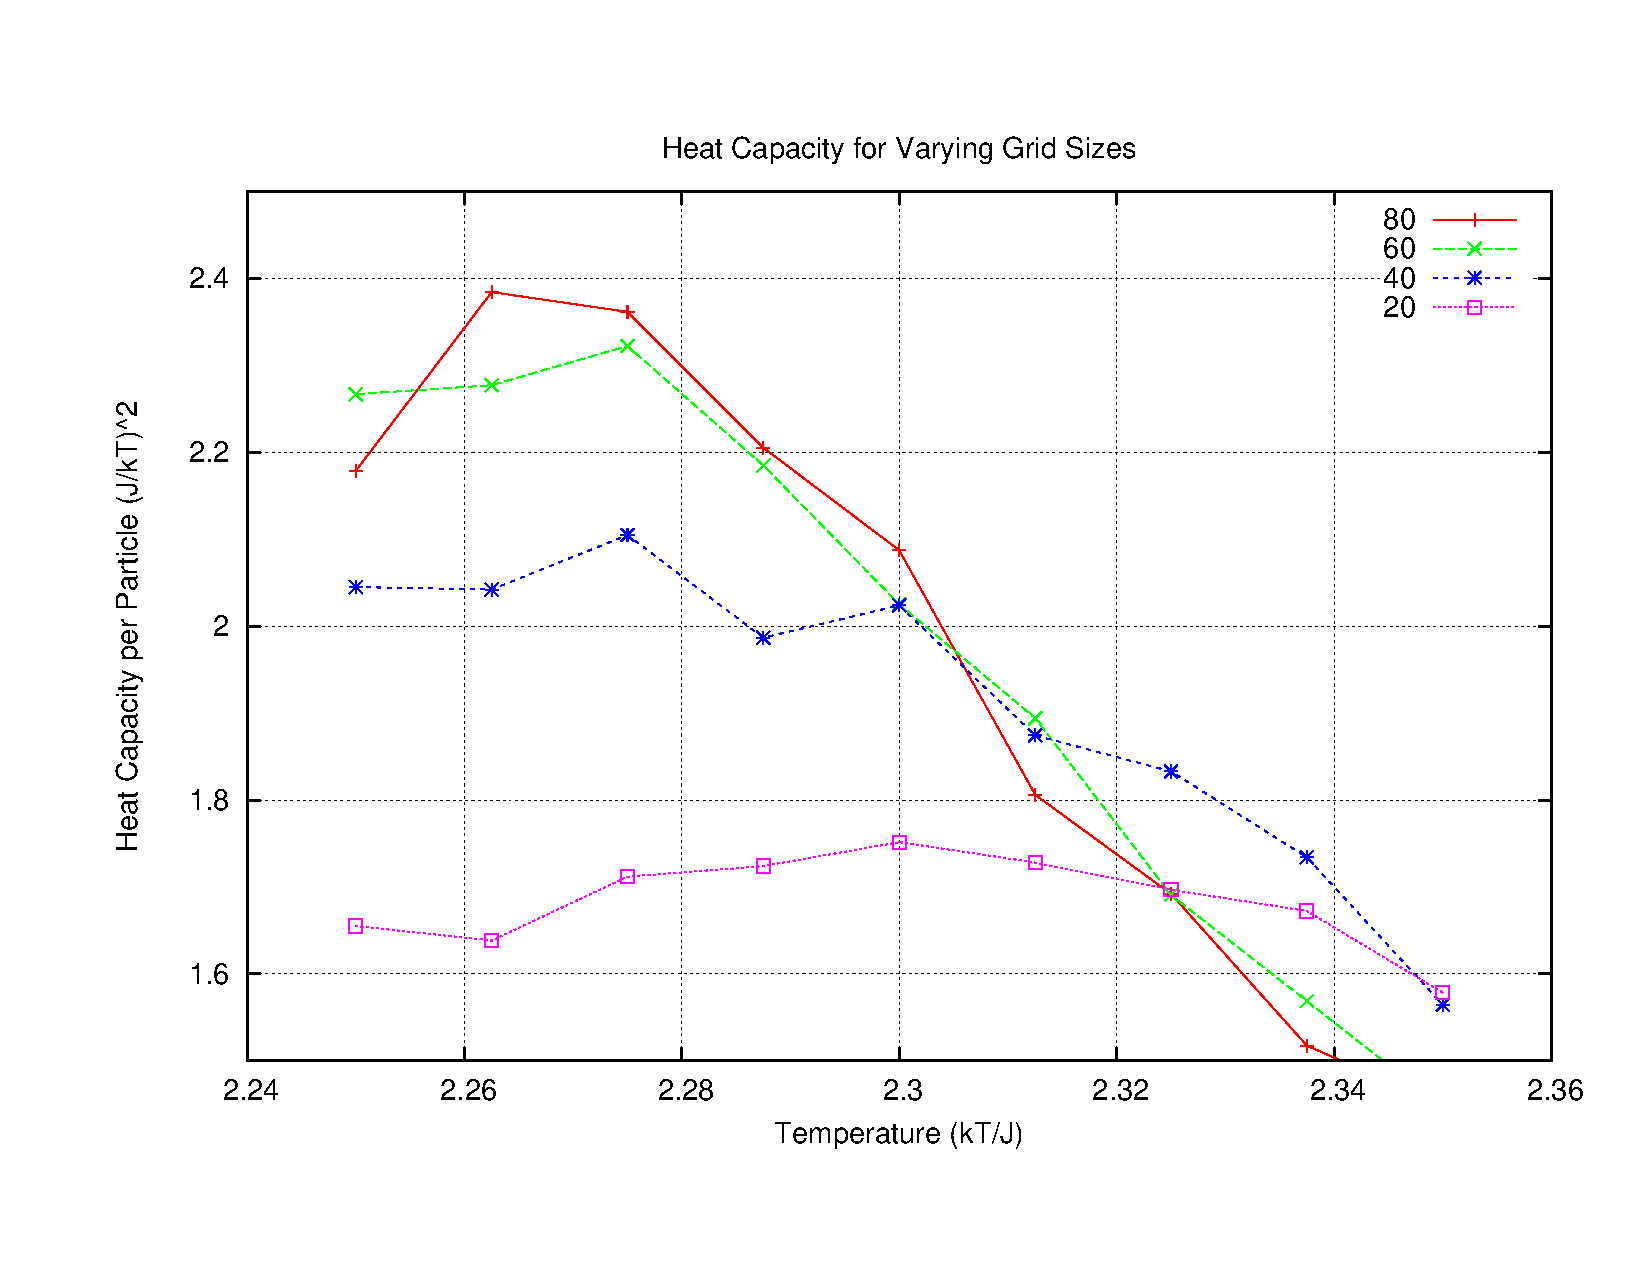
\includegraphics[width=1.0\textwidth]{heatcapacity_zoom.pdf}
\caption{Here we have calculated the heat capacity with a finer step size between T=2.25 and T=2.35 for varying grid sizes. We note that the location of each peak corresponds to a phase transition and mark each critical temperature in Figure (15) in order to find $T_c$ in the infinite grid size limit.}
\end{figure}
\begin{figure}
\centering
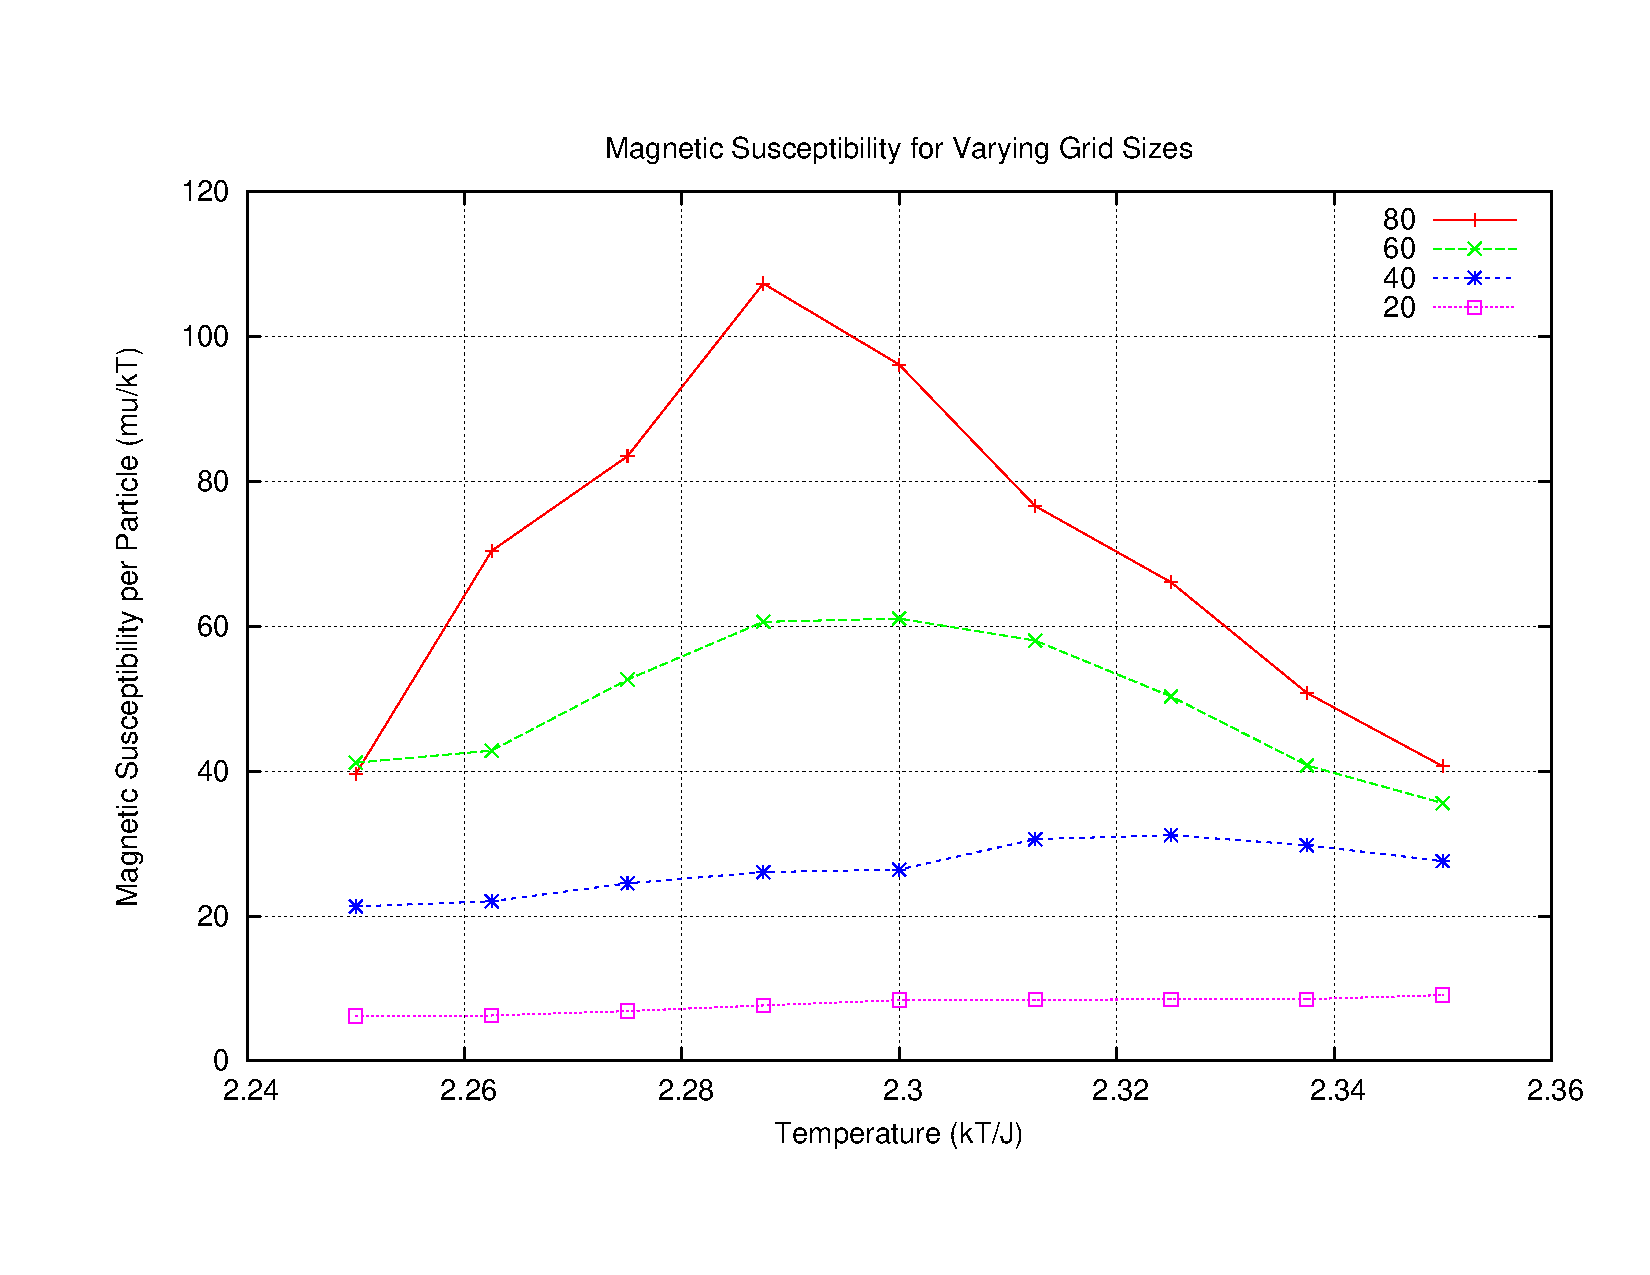
\includegraphics[width=1.0\textwidth]{magsus_zoom.pdf}
\caption{Here we have calculated the magnetic susceptibility with a finer step size between T=2.25 and T=2.35 for varying grid sizes. We note that the location of each peak corresponds to a phase transition and mark each critical temperature in Figure (15) in order to find $T_c$ in the infinite grid size limit.}
\end{figure}
\begin{figure}
\centering
\begin{tabular}{| l | l | l |}
\hline
Grid Size & $T_c (C_v)$ & $T_c (\chi)$ \\ \hline
20	&	2.3		& 2.35 \\ \hline
40 	&	2.275	& 2.325 \\ \hline
60 	&	2.275	& 2.3 \\ \hline
80	&	2.2625	& 2.2875	\\ \hline
\end{tabular}
\caption{Here we have compiled the observed critical temperatures for increasing grid sizes. We note that as the grid size increases, the critical temperature approaches the exact result of $T_c (n \rightarrow \infty) \approx$ 2.269.}
\end{figure}
\begin{figure}
\centering
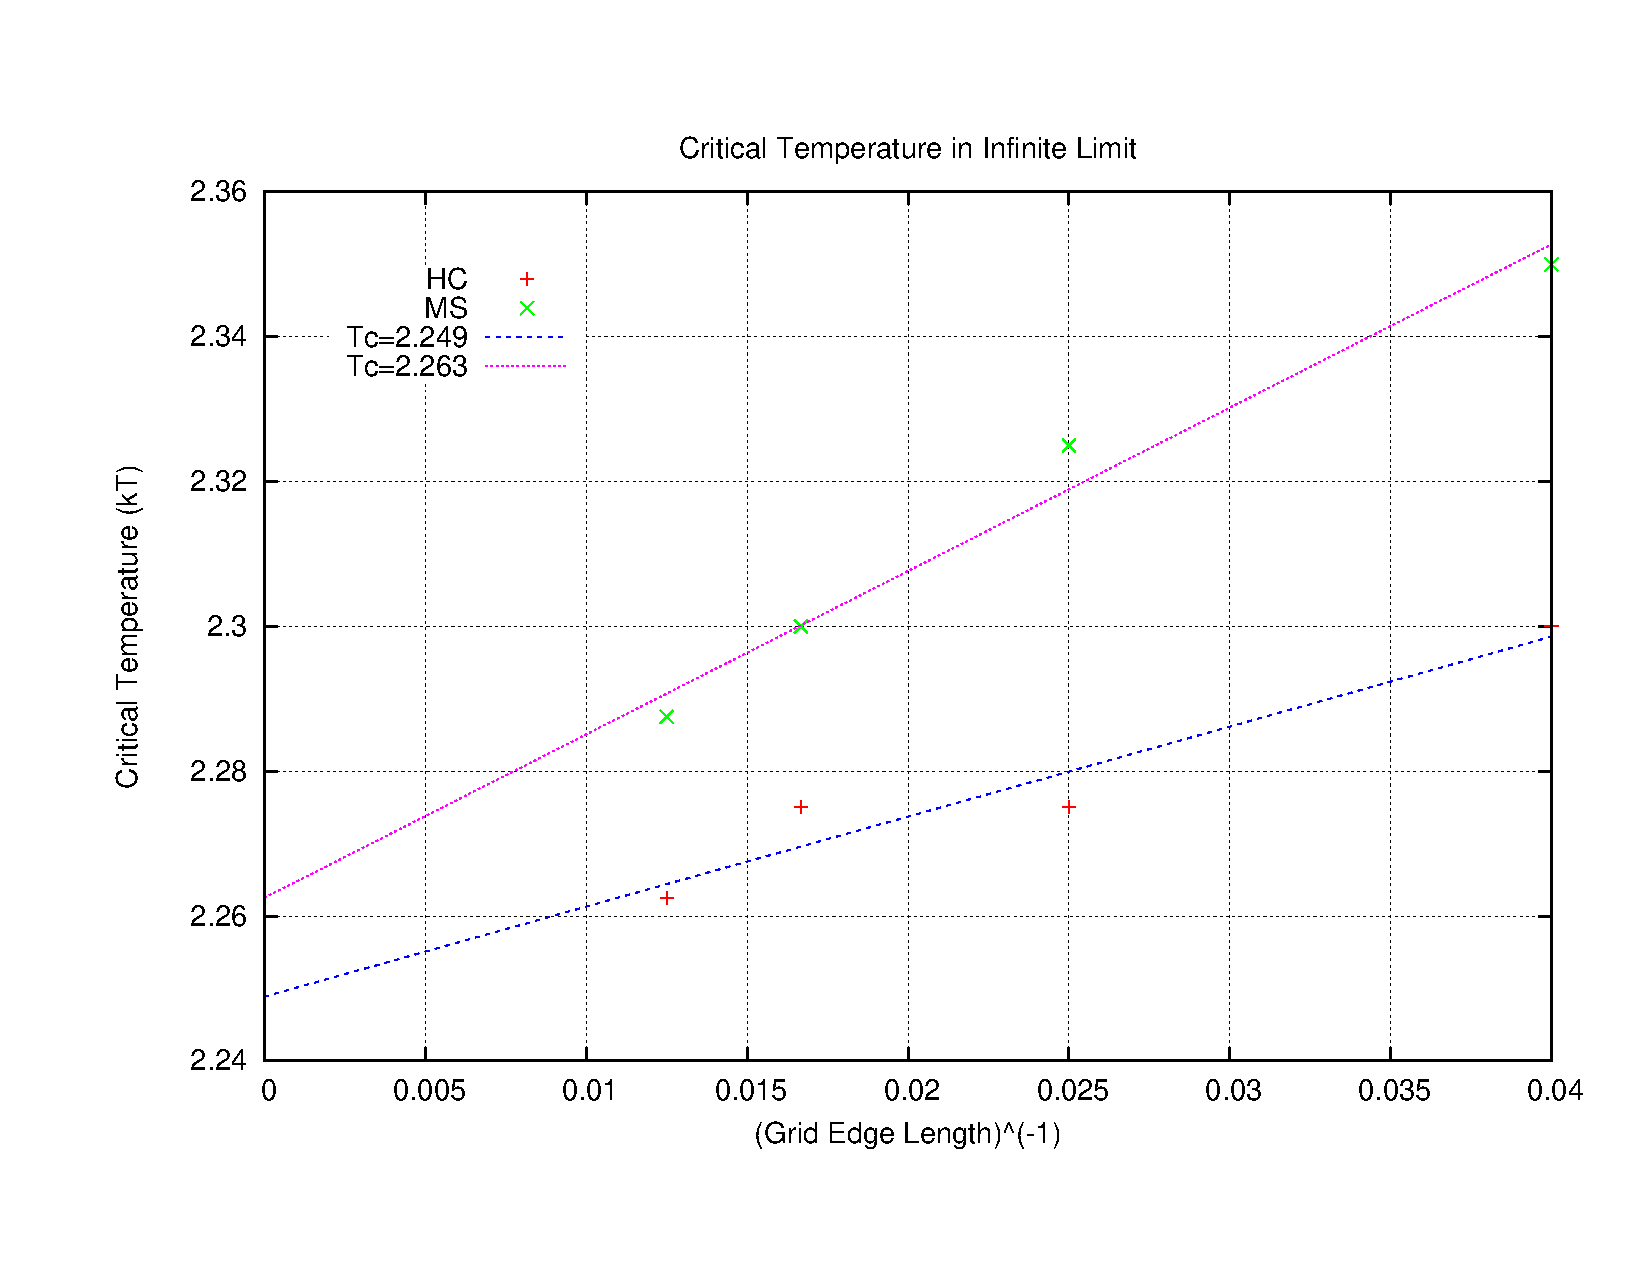
\includegraphics[width=1.0\textwidth]{crittemp.pdf}
\caption{Here we have plotted $T_c$ as a function of $\frac{1}{n}$ in order to find $T_c$ in the infinite limit. As $n \rightarrow \infty$, $\frac{1}{n} \rightarrow 0$ and $T_c$ will approach the exact solution. From curve fitting the lines, we obtain from the heat capacity that $T_c(n\rightarrow \infty)$ = 2.248 $\pm$ 0.007 and from the magnetic susceptibility that $T_c(n\rightarrow \infty)$ = 2.263 $\pm$ 0.007. We see that the prediction from the magnetic susceptibility agrees within error with the exact result of 2.269.}
\end{figure}


\section{Discussion}

Here we discuss the accuracy and speed of the algorithm, followed by investigations into varying grid sizes that may find the critical temperature in the infinite limit.

From Figure (1), we see that while the mean energy and mean magnetization may be found with a number of monte carlo cycles on the order of $2^{10} - 2^{15}$, agreement for the heat capacity and magnetic susceptibility requires monte carlo counts on the order of $2^{18} - 2^{20}$. From Figure (2) we see that the program scales linearly with the number of required operations, both with the number of spins and number of monte carlo cycles. A tenfold increase in grid size results in a hundredfold increase in the number of spins and a hundredfold increase in computation time. Similarly, a tenfold increase in the number of monte carlo cycles results in a tenfold increase in computation time. From Figures (3) and (4) we see that degree of alignment greatly affects the number of monte carlo cycles required before equilibrium is reached. Full alignment for low temperatures and random alignment for high temperatures lead to lower required counts. From Figure (5) we see that the number of accepted states increases with higher temperatures. From Figures (6) and (7) we observe that the center of the probability distribution shifts from $E$/N = -2 for low temperatures toward $E$/N = 0 for high temperatures.

From Figures (8) through (11) we observe the indications of a phase transition. In the mean energy and mean magnetizatin we see a change in the concavity of the graph and in the heat capacity and magnetic susceptibility we see a peaking of the respective values, each indicative of a phase transition. In order to better find the critical temperatures from these graphs, we replot the heat capacity and magnetic susceptibility in Figures (12) and (13), respectively, with finer steps in temperature. Listing the temperature values corresponding to the peaks as the critical temperatures, Figure (14), we plot the values as a function of one over grid size. From the intercept of each line we are finally able to extract the critical temperature in the infinite limit; the exact solution is $T_c \approx$ 2.269. The heat capacity giving 2.248 $\pm$ 0.007 and the magnetic susceptibility 2.263 $\pm$ 0.007, the latter clearly lying within error of the exact solution. 

\section{Conclusion}

In this project I develop an algorithm which reproduces the 2D Ising Model for a given grid size and temperature. The code scales linearly with the number of spins and the number of monte carlo cycles; it is reasonably fast for small grid sizes, but it quickly scales to multiple minute computation times for grid sizes approaching one hundred. The algorithm reproduces well the exact solutions from the two-by-two case with $2^20$ monte carlo cycles. By investigating larger grid sizes, 20, 40, 60, and 80, we found the indications of a phase transition; by plotting these against one over the grid size we approximated the infinite solution from the intercept of a linear fit. The magnetic susceptibility fit reproduced the infinite limit within error, with 2.263 $\pm$ 0.007 compared to 2.269 for the exact solution.

\section{References}

[1] M. Hjorth-Jensen. Computational Physics, lecture notes spring 2016. Department of Physics, Michigan State University, 2016. \newline

\newpage

\section*{Code Attachment}

\begin{lstlisting}[title={project4.cpp}]
#include<iostream>
#include<iomanip>
#include<cmath>
#include<fstream>
#include<random>
#include<chrono>
#include "time.h"
#include "project4_library.h"
#include "spinsystem_library.h"

using namespace std;

ofstream ofile;

int main(int argc, char* argv[]){
	int i, n, accstates, cycles, align, printcount, cycpow, choice;
	double T, J, time, current_T;
	char* outfilename, *probfilename;
	clock_t start, finish;

	/**************************************************
	Enter required information via command line
		n = grid size
		T = temperature
			choice = 0; choice = 1
				T = exact temperature
				T = number of temp steps between
					Tmin and Tmax
		J = energy
		align
			= 0		random orientation
			= 1		fully aligned (up)
			= 2		keep alignment from previous
						computation
		outfilename = output file name
		cycles = power of 2 for number of MC cycles
					So 	5 ---> 2^5
						6 ---> 2^6
						etc
		choice (prob_write_temp) 
			= 0 	probability distribution file
			= 1		loop through cycles count
						2^0 ---> 2^entry
			= 2		loop through temperature
						Enter Tmin, Tmax
						T = steps from Tmin to Tmax
						Tmin + i*(Tmax-Tmin)/T
						Tmin ... Tmax in T+1 steps
	**************************************************/
	if(argc<8){
		cout << "Bad usage. Enter also 'n T J aligned_init_0_1_2 outfilename cycles prob_write_temp_0_1_2' on same line." << endl;
		exit(1);
	}
	else{
		n = atoi(argv[1]);
		T = atof(argv[2]);
		J = atof(argv[3]);
		align = atoi(argv[4]);
		outfilename = argv[5];
		cycles = atoi(argv[6]);
		choice = atoi(argv[7]);
	}


	/**************************************************
	Create and initialize nxn spin grid; calculate
		energy, magnetization, etc.
	**************************************************/
	spin_system spinbaby(n,n,J,T);
	if(align==1){
		spinbaby.align_up();
	}

	/**************************************************
	Create spin_evolution from the spin_system
	**************************************************/
	spin_evolution spinadult(spinbaby);


	/**************************************************
	Evolve according to choice value
		0 ---> probability
		1 ---> loop through cycle counts
		2 ---> loop through temperature values
				in T+1 steps, including Tmin, Tmax
	**************************************************/
	if(choice==0){
		start = clock();

		cycpow = pow(2,cycles);

		/**************************************************
			evolve through 2^cycles
			track the number of accepted states
			Note: we do this so the equilibrium is reached
					before computation
		**************************************************/
		spinadult.evolution(accstates, cycpow);

		cout << endl;
		cout << cycles << setw(15) << accstates;

		spinadult.print();

		finish = clock();
		time = (finish - start)/((double) CLOCKS_PER_SEC);

		cout << "time" << endl;
		cout << setw(15) << time << endl;

		/**************************************************
			reset statistics in spin_evolution now
				that equilibrium has been reached
		**************************************************/
		spinadult.reset_statistics();

		cycpow = pow(2,cycles);
		spinadult.evolution(accstates, cycpow);

		ofile.open(outfilename);
		ofile << setw(15) << "#E" << setw(15) << "E/N" << setw(15) << "Prob" <<  setw(15) << "count" << endl;
		for(i=0;i<2*n*n + 1; i++){
			ofile << setw(15) << (i-n*n)*2 << setw(15) << (double) ((i-n*n)*2)/(double) (n*n);
			ofile << setw(15) << (double) spinadult.probability[i]/(double) cycpow << setw(15) << spinadult.probability[i] << endl;
		}
		ofile.close();
	}
	else if(choice==1){
		ofile.open(outfilename);
		ofile << setw(15) << "#i" << setw(15) << "cyc" << setw(15) << "accs" << setw(15) << "time";
		ofile << setw(15) << "<E>" << setw(15) << "e_v" << setw(15) << "<M>" << setw(15) << "m_v";
		ofile << setw(15) << "<|M|>" << setw(15) << "m_abs_v" << setw(15) << "Cv" << setw(15) << "Khi" << endl;
		for(i=0;i<cycles+1;i++){
			/**************************************************
				Align according to choice for each loop
				reset stastics before calculations begin
			**************************************************/
			if(align==0){
				spinadult.spintoddler.randomize();
			}
			else if(align==1){
				spinadult.spintoddler.align_up();
			}
			spinadult.reset_statistics();

			start = clock();

			/**************************************************
				Evolve over 2^cycles MC
			**************************************************/
			cycpow = pow(2,i);
			spinadult.evolution(accstates, cycpow);

			finish = clock();
			time = (finish - start)/((double) CLOCKS_PER_SEC);

			ofile << setw(15) << i << setw(15) << cycpow << setw(15) << accstates << setw(15) << time;
			ofile << setw(15) << spinadult.energy_mean << setw(15) << spinadult.e_variance;
			ofile << setw(15) << spinadult.magn_mean << setw(15) << spinadult.m_variance;
			ofile << setw(15) << spinadult.magn_mean_abs << setw(15) << spinadult.m_abs_variance;
			ofile << setw(15) << spinadult.heat_capacity << setw(15) << spinadult.susceptibility << endl;
			cout << setw(15) << i << setw(15) << cycpow << setw(15) << time << " seconds" << endl;
		}
		ofile.close();
	}
	else if(choice==2){
		ofile.open(outfilename);
		ofile << "#T" << setw(15) << "time" << setw(15) << "accs";
		ofile << setw(15) << "<E>" << setw(15) << "e_v" << setw(15) << "<M>" << setw(15) << "m_v";
		ofile << setw(15) << "<|M|>" << setw(15) << "m_abs_v" << setw(15) << "Cv" << setw(15) << "Khi" << endl;

		/**************************************************
			input Tmin and Tmax
		**************************************************/
		double Tm, TM;
		cout << "Enter Tmin: ";
		cin >> Tm;
		cout << "Enter Tmax: ";
		cin >> TM;

		/**************************************************
			align as chosen
		**************************************************/
		cycpow = pow(2,cycles);
		if(align==0){
			spinadult.spintoddler.randomize();
		}
		else if(align==1){
			spinadult.spintoddler.align_up();
		}
		else if(align==2){
			spinadult.evolution(accstates, cycpow);
		}

		for(i=0;i<T+1;i++){
			/**************************************************
				Calculate T for this iteration
				reset statistics
				evolve
			**************************************************/
			start = clock();
			current_T = Tm + ((TM-Tm)/T)*(double)i;
			spinadult.spintoddler.T = current_T;
			spinadult.reset_statistics();
			spinadult.evolution(accstates, cycpow);
			finish = clock();
			time = (finish - start)/((double) CLOCKS_PER_SEC);
			ofile << current_T << setw(15) << time << setw(15) << accstates;
			ofile << setw(15) << spinadult.energy_mean << setw(15) << spinadult.e_variance;
			ofile << setw(15) << spinadult.magn_mean << setw(15) << spinadult.m_variance;
			ofile << setw(15) << spinadult.magn_mean_abs << setw(15) << spinadult.m_abs_variance;
			ofile << setw(15) << spinadult.heat_capacity << setw(15) << spinadult.susceptibility << endl;
			cout << setw(15) << current_T << setw(15) << accstates << setw(15) << time << " seconds" << endl;
		}
		ofile.close();
	}

	return 0;
}
\end{lstlisting}
\begin{lstlisting}[title={project4-library.h}]
#ifndef PROJECT4_LIBRARY_H
#define PROJECT4_LIBRARY_H

#include<iostream>
#include<iomanip>
#include<cmath>
#include<fstream>
#include<random>
#include<chrono>
#include "time.h"

using namespace std;

ofstream spinfile;

void array_alloc(double*& a, int length);
void array_delete(double*& a);
void matrix_alloc(int**& A, int rows, int columns);
void matrix_delete(int**& A, int rows);
void matrix_print(int**& A, int rows, int columns);

void array_alloc(double*& a, int length){
	a = new double[length];
}
void array_delete(double*& a){
	delete[] a;
}
void matrix_alloc(int**& A, int rows, int columns){
	int i, j;
	A = new int*[rows];
	for(i=0;i<rows;i++){
		A[i] = new int[columns];
	}
	for(i=0;i<rows;i++){
		for(j=0;j<columns;j++){
			A[i][j] = 0.0;
		}
	}
}
void matrix_delete(int**& A, int rows){
	int i;
	for(i=0;i<rows;i++){
		delete[] A[i];
	}
	delete[] A;
}
void matrix_print(int**& A, int rows, int columns){
	int i, j;
	for(i=0;i<rows;i++){
		for(j=0;j<columns;j++){
			cout << setw(10) << A[i][j];
		}
		cout << endl;
	}
}

#endif
\end{lstlisting}
\begin{lstlisting}[title={spinsystem-library.h}]
#ifndef SPINSYSTEM_LIBRARY_H
#define SPINSYSTEM_LIBRARY_H

#include<iostream>
#include<iomanip>
#include<cmath>
#include<fstream>
#include<random>
#include<chrono>
#include "time.h"

using namespace std;

class spin_system{
	public:
		int** spin;
		int rows, columns;
		double J, T;
		double energy, magnetization;

		spin_system();
		spin_system(int,int,double,double);
		spin_system(int,int,double,double,int);

		void print();
		void energy_total();
		void magnetization_total();
		void randomize();
		void align_up();
		void align_down();
};
class spin_evolution{
	public:
		spin_system spintoddler;
		int* probability;
		double exponential[2];
		double energy_mean, energy_sq_mean;
		double heat_capacity, e_variance;
		double magn_mean, magn_mean_abs, magn_sq_mean;
		double susceptibility, m_variance, m_abs_variance;
		
		spin_evolution(spin_system&);

		void energy_change_check(double&,int&,int,int);
		void evolve_test(bool&,double,int);
		void evolve_test1(bool&,double,int,double);
		void evolve(double,int,int);
		void metropolis(int&);
		void metropolis1(int&);
		void update_statistics();
		void reset_statistics();
		void final_form(int);
		void evolution(int&,int);
		void print();
};

spin_evolution::spin_evolution(spin_system& spinbaby){
	int i, j;	
	spintoddler.rows = spinbaby.rows;
	spintoddler.columns = spinbaby.columns;
	spintoddler.J = spinbaby.J;
	spintoddler.T = spinbaby.T;
	spintoddler.energy = spinbaby.energy;
	spintoddler.magnetization = spinbaby.magnetization;
	
	spintoddler.spin = new int*[spintoddler.rows];
	for(i=0;i<spintoddler.rows;i++){
		spintoddler.spin[i] = new int[spintoddler.columns];
	}

	for(i=0;i<spintoddler.rows;i++){
		for(j=0;j<spintoddler.columns;j++){
			spintoddler.spin[i][j] = spinbaby.spin[i][j];
		}
	}
	probability = new int[4*spintoddler.rows*spintoddler.columns+1];
	for(i=0;i<2*spintoddler.rows*spintoddler.columns+1;i++){
		probability[i] = 0;
	}

	exponential[0] = exp(-4.0*spintoddler.J/spintoddler.T);
	exponential[1] = exp(-8.0*spintoddler.J/spintoddler.T);

	energy_mean = 0.0; energy_sq_mean = 0.0;
	heat_capacity = 0.0; e_variance = 0.0;
	magn_mean = 0.0; magn_mean_abs = 0.0; magn_sq_mean = 0.0;
	susceptibility = 0.0; m_variance = 0.0; m_abs_variance = 0.0;
}
void spin_evolution::energy_change_check(double& delta_e, int& index, int x, int y){
	int n, m;
	double sum;
	n = spintoddler.rows;
	m = spintoddler.columns;
	sum = (spintoddler.spin[(x+1)%n][y] + spintoddler.spin[(x+n-1)%n][y] + spintoddler.spin[x][(y+1)%m] + spintoddler.spin[x][(y+m-1)%m]);
	delta_e = 0;
	if(sum==0){}
	else{
		delta_e = 2.0*((double) spintoddler.spin[x][y])*sum;
		index = abs(sum)/2 - 1;
	}
}	
void spin_evolution::evolve_test(bool& test, double delta_e, int index){
	double random;
	unsigned seed;

	test = false;

	seed = chrono::system_clock::now().time_since_epoch().count();
	default_random_engine generator (seed);
	uniform_real_distribution<double> double_dist(0.0,1.0);

	if(delta_e>0){
		random = double_dist(generator);
		if(random > exponential[index]){
			//faster to check > than both < and =
		}
		else{
			test = true;
		}
	}
	else{
		test = true;
	}
}		
void spin_evolution::evolve(double delta_e, int x, int y){
	spintoddler.spin[x][y] *= -1;
	spintoddler.magnetization += 2*spintoddler.spin[x][y];
	spintoddler.energy += delta_e;
}
void spin_evolution::update_statistics(){
	int index;
	energy_mean += spintoddler.energy;
	energy_sq_mean += spintoddler.energy*spintoddler.energy;
	magn_mean += spintoddler.magnetization;
	magn_mean_abs += abs(spintoddler.magnetization);
	magn_sq_mean += spintoddler.magnetization*spintoddler.magnetization;
	index = spintoddler.energy/2 + spintoddler.rows*spintoddler.columns;
	probability[index] += 1;
}
void spin_evolution::reset_statistics(){
	int i;	
	energy_mean = 0.0;
	magn_mean = 0.0;
	magn_mean_abs = 0.0;
	energy_sq_mean = 0.0;
	magn_sq_mean = 0.0;

	e_variance = 0.0;
	heat_capacity = 0.0;
	m_variance = 0.0;
	m_abs_variance = 0.0;
	susceptibility = 0.0;

	for(i=0;i<2*spintoddler.rows*spintoddler.columns+1;i++){
		probability[i] = 0;
	}

	exponential[0] = exp(-4.0*spintoddler.J/spintoddler.T);
	exponential[1] = exp(-8.0*spintoddler.J/spintoddler.T);
}
void spin_evolution::final_form(int cycles){
	double T, spins, cycles_d;
	T = spintoddler.T;
	spins = spintoddler.rows*spintoddler.columns;
	cycles_d = cycles;

	energy_mean /= cycles_d;
	magn_mean /= cycles_d;
	magn_mean_abs /= cycles_d;
	energy_sq_mean /= cycles_d;
	magn_sq_mean /= cycles_d;

	e_variance = (energy_sq_mean - energy_mean*energy_mean)/spins;
	heat_capacity = e_variance/T/T;
	m_variance = (magn_sq_mean - magn_mean*magn_mean)/spins;
	m_abs_variance = (magn_sq_mean - magn_mean_abs*magn_mean_abs)/spins;
	susceptibility = m_abs_variance/T;

	energy_mean /= spins;
	magn_mean /= spins;
	magn_mean_abs /= spins;
	energy_sq_mean /= spins;
	magn_sq_mean /= spins;
}	
void spin_evolution::metropolis(int& accstates){
	bool test;

	int i, x, y, spins, index;
	spins = spintoddler.rows*spintoddler.columns;

	double delta_e, random;

	unsigned seed;

	//Random number generators
	seed = chrono::system_clock::now().time_since_epoch().count();
	default_random_engine generator (seed);
	uniform_int_distribution<int> int_x(0,spintoddler.rows-1);
	uniform_int_distribution<int> int_y(0,spintoddler.columns-1);

	for(i=0;i<spins;i++){
		x = int_x(generator); y = int_y(generator);
		energy_change_check(delta_e, index, x, y);
		evolve_test(test, delta_e, index);
		if(test==true){
			evolve(delta_e,x,y);
			accstates++;
		}
	}
}	
void spin_evolution::evolution(int& accstates, int cycles){
	int i;
	accstates = 0;

	for(i=0;i<cycles;i++){
		metropolis(accstates);
		update_statistics();
	}
	final_form(cycles);
}
void spin_evolution::print(){
	int i;
	spintoddler.print();
	cout << "<E>/N" << endl;
	cout << setw(15) << energy_mean << " +/- " << pow(e_variance,0.5) << endl;
	cout << "<M>/N" << endl;
	cout <<	setw(15) << magn_mean << " +/- " << pow(m_variance,0.5) << endl;
	cout << "<|M|>/N" << endl;
	cout << setw(15) << magn_mean_abs << " +/- " << pow(m_abs_variance,0.5) << endl;
	cout << "Cv/N" << endl;
	cout << setw(15) << heat_capacity << endl;
	cout << "Khi/N" << endl;
	cout << setw(15) << susceptibility << endl;
	cout << endl;
}

/********************
	SPIN_SYSTEM
********************/

spin_system::spin_system(){
	rows = 0; columns = 0;
	energy = 0;
	magnetization = 0;
	J = 0;
	T = 0;
}
spin_system::spin_system(int x, int y, double J0, double T0){
	int i, j;

	unsigned seed = chrono::system_clock::now().time_since_epoch().count();
	default_random_engine generator (seed);
	uniform_int_distribution<int> distribution(0,1);

	J = J0; T = T0;
	rows = x; columns = y;

	spin = new int*[rows];
	for(i=0;i<rows;i++){
		spin[i] = new int[columns];
	}

	for(i=0;i<rows;i++){
		for(j=0;j<columns;j++){
			spin[i][j] = distribution(generator);
			if(spin[i][j]==0){
				spin[i][j] = -1;
			}
		}
	}
	magnetization_total();
	energy_total();
}
spin_system::spin_system(int x, int y, double J0, double T0, int align){
	int i, j;

	J = J0; T = T0;
	rows = x; columns = y;

	spin = new int*[rows];
	for(i=0;i<rows;i++){
		spin[i] = new int[columns];
	}

	for(i=0;i<rows;i++){
		for(j=0;j<columns;j++){
			spin[i][j] = align;
		}
	}
	magnetization = rows*columns*align;
	energy = -rows*columns*2.0*J;
}
void spin_system::print(){
	int i, j;
	cout << endl;
	for(i=0;i<rows;i++){
		for(j=0;j<columns;j++){
			cout << setw(5) << spin[i][j];
		}
		cout << endl;
	}
	cout << "energy" << endl;
	cout << setw(15) << energy << endl;
	cout << "magnetization" << endl;
	cout << setw(15) << magnetization << endl;
	cout << endl;
}
void spin_system::energy_total(){
	int i, j;
	energy = 0;
	for(i=0;i<rows;i++){
		for(j=0;j<columns;j++){
			energy += -spin[i][j]*(spin[(i+1)%rows][j] + spin[(i+rows-1)%rows][j] + spin[i][(j+1)%columns] + spin[i][(j+columns-1)%columns]);
		}
	}
	energy /= 2.0;
}
void spin_system::magnetization_total(){
	int i, j;
	magnetization = 0.0;
	for(i=0;i<rows;i++){
		for(j=0;j<columns;j++){
			magnetization += spin[i][j];
		}
	}
}
void spin_system::randomize(){
	int i, j;
	unsigned seed = chrono::system_clock::now().time_since_epoch().count();
	default_random_engine generator (seed);
	uniform_int_distribution<int> distribution(0,1);
	magnetization = 0;
	for(i=0;i<rows;i++){
		for(j=0;j<columns;j++){
			spin[i][j] = distribution(generator);
			if(spin[i][j]==0){
				spin[i][j] = -1;
			}
			magnetization += spin[i][j];
		}
	}
	energy_total();
}
void spin_system::align_up(){
	int i, j;
	for(i=0;i<rows;i++){
		for(j=0;j<columns;j++){
			spin[i][j] = 1;
		}
	}
	magnetization = rows*columns;
	energy = -rows*columns*2;
}
void spin_system::align_down(){
	int i, j;
	for(i=0;i<rows;i++){
		for(j=0;j<columns;j++){
			spin[i][j] = -1;
		}
	}
	magnetization = -rows*columns;
	energy = -rows*columns*2;
}


#endif
\end{lstlisting}
\end{document}

